\subsection{Fundamentos}

	Cuando se trabaja con sensores con ruido de media desconocida, no nula y constante, nuestro modelo es el siguiente:

	\begin{equation*}
		\vect{\eta_{n}} = \vect{\tilde{\eta}_{n}} + \vect{\mu}
	\end{equation*}

	\begin{equation*}
		\Sigma_{d}:
		\begin{cases}
			\vect{x_{n + 1}} = A_{d}\: \vect{x_{n}} + B_{d} \: \vect{\xi_{n}} \\
			\vect{y_{n}} = C_{d}\: \vect{x_{n}} + \vect{\tilde{\eta}_{n}} + \vect{\mu}
		\end{cases}
	\end{equation*}

	Donde ahora el nuevo ruido $\vect{\tilde{\eta}_{n}}$ es de media nula, y se representa la media del ruido como $\vect{\mu}$. Una técnica para llevar el nuevo modelo a la forma del modelo anterior consiste en considerar la media del ruido como un estado más a estimar. De esta forma se incluye dentro de las variables de estado:

	\begin{equation*}
		\vect{z}_{n} = \begin{bmatrix} \vect{x}_{n} \\[0.3em] \vect{\mu}\end{bmatrix} \qquad%
	\end{equation*}
	
	Y el nuevo modelo es:
	
	\begin{equation*}
		\tilde{\Sigma_{d}}:
		\begin{cases}
			\vect{z_{n + 1}} = \tilde{A_{d}}\: \vect{z_{n}} + \tilde{B_{d}} \: \vect{\xi_{n}} \\
			\vect{y_{n}} = \tilde{C_{d}}\: \vect{z_{n}} + \vect{\tilde{\eta}_{n}}
		\end{cases}
	\end{equation*}

	Con las nuevas matrices:
	
	\begin{equation*}
			\tilde{A_{d}} = \begin{bmatrix} A_{d} & 0 \\[0.3em] 0 & I \end{bmatrix}
	\end{equation*}
	
	\begin{equation*}
			\tilde{B_{d}} = \begin{bmatrix} B_{d} \\[0.3em] 0 \end{bmatrix}
	\end{equation*}
	
	\begin{equation*}
			\tilde{C_{d}} = \begin{bmatrix} C_{d} & I \end{bmatrix}
	\end{equation*}
	
	Cabe aclarar que el éxito de esta solución dependerá de la observabilidad del nuevo sistema. A continuación se expondrán las distintas variantes que pueden darse en cuanto a la observabilidad.

%--------------------------------------------------------------------------------------------------

\subsection{Medición de P - Sesgo en P}

	En la figura \ref{fig:ej4a} se observa el resultado de medir sólo posición, con un sesgo en la misma. En el gráfico sin la estimación del sesgo, la estimación de la trayectoria se encuentra desviada de la real, de la misma manera que lo estan las mediciones. Cuando se trata de estimar el sesgo, el resultado mejora pero no sigue la trayectoria con la misma efectividad que lo hacia en puntos anteriores donde no había sesgo, problema ligado a la observabilidad.

	\begin{figure}[H]
		\centering
		%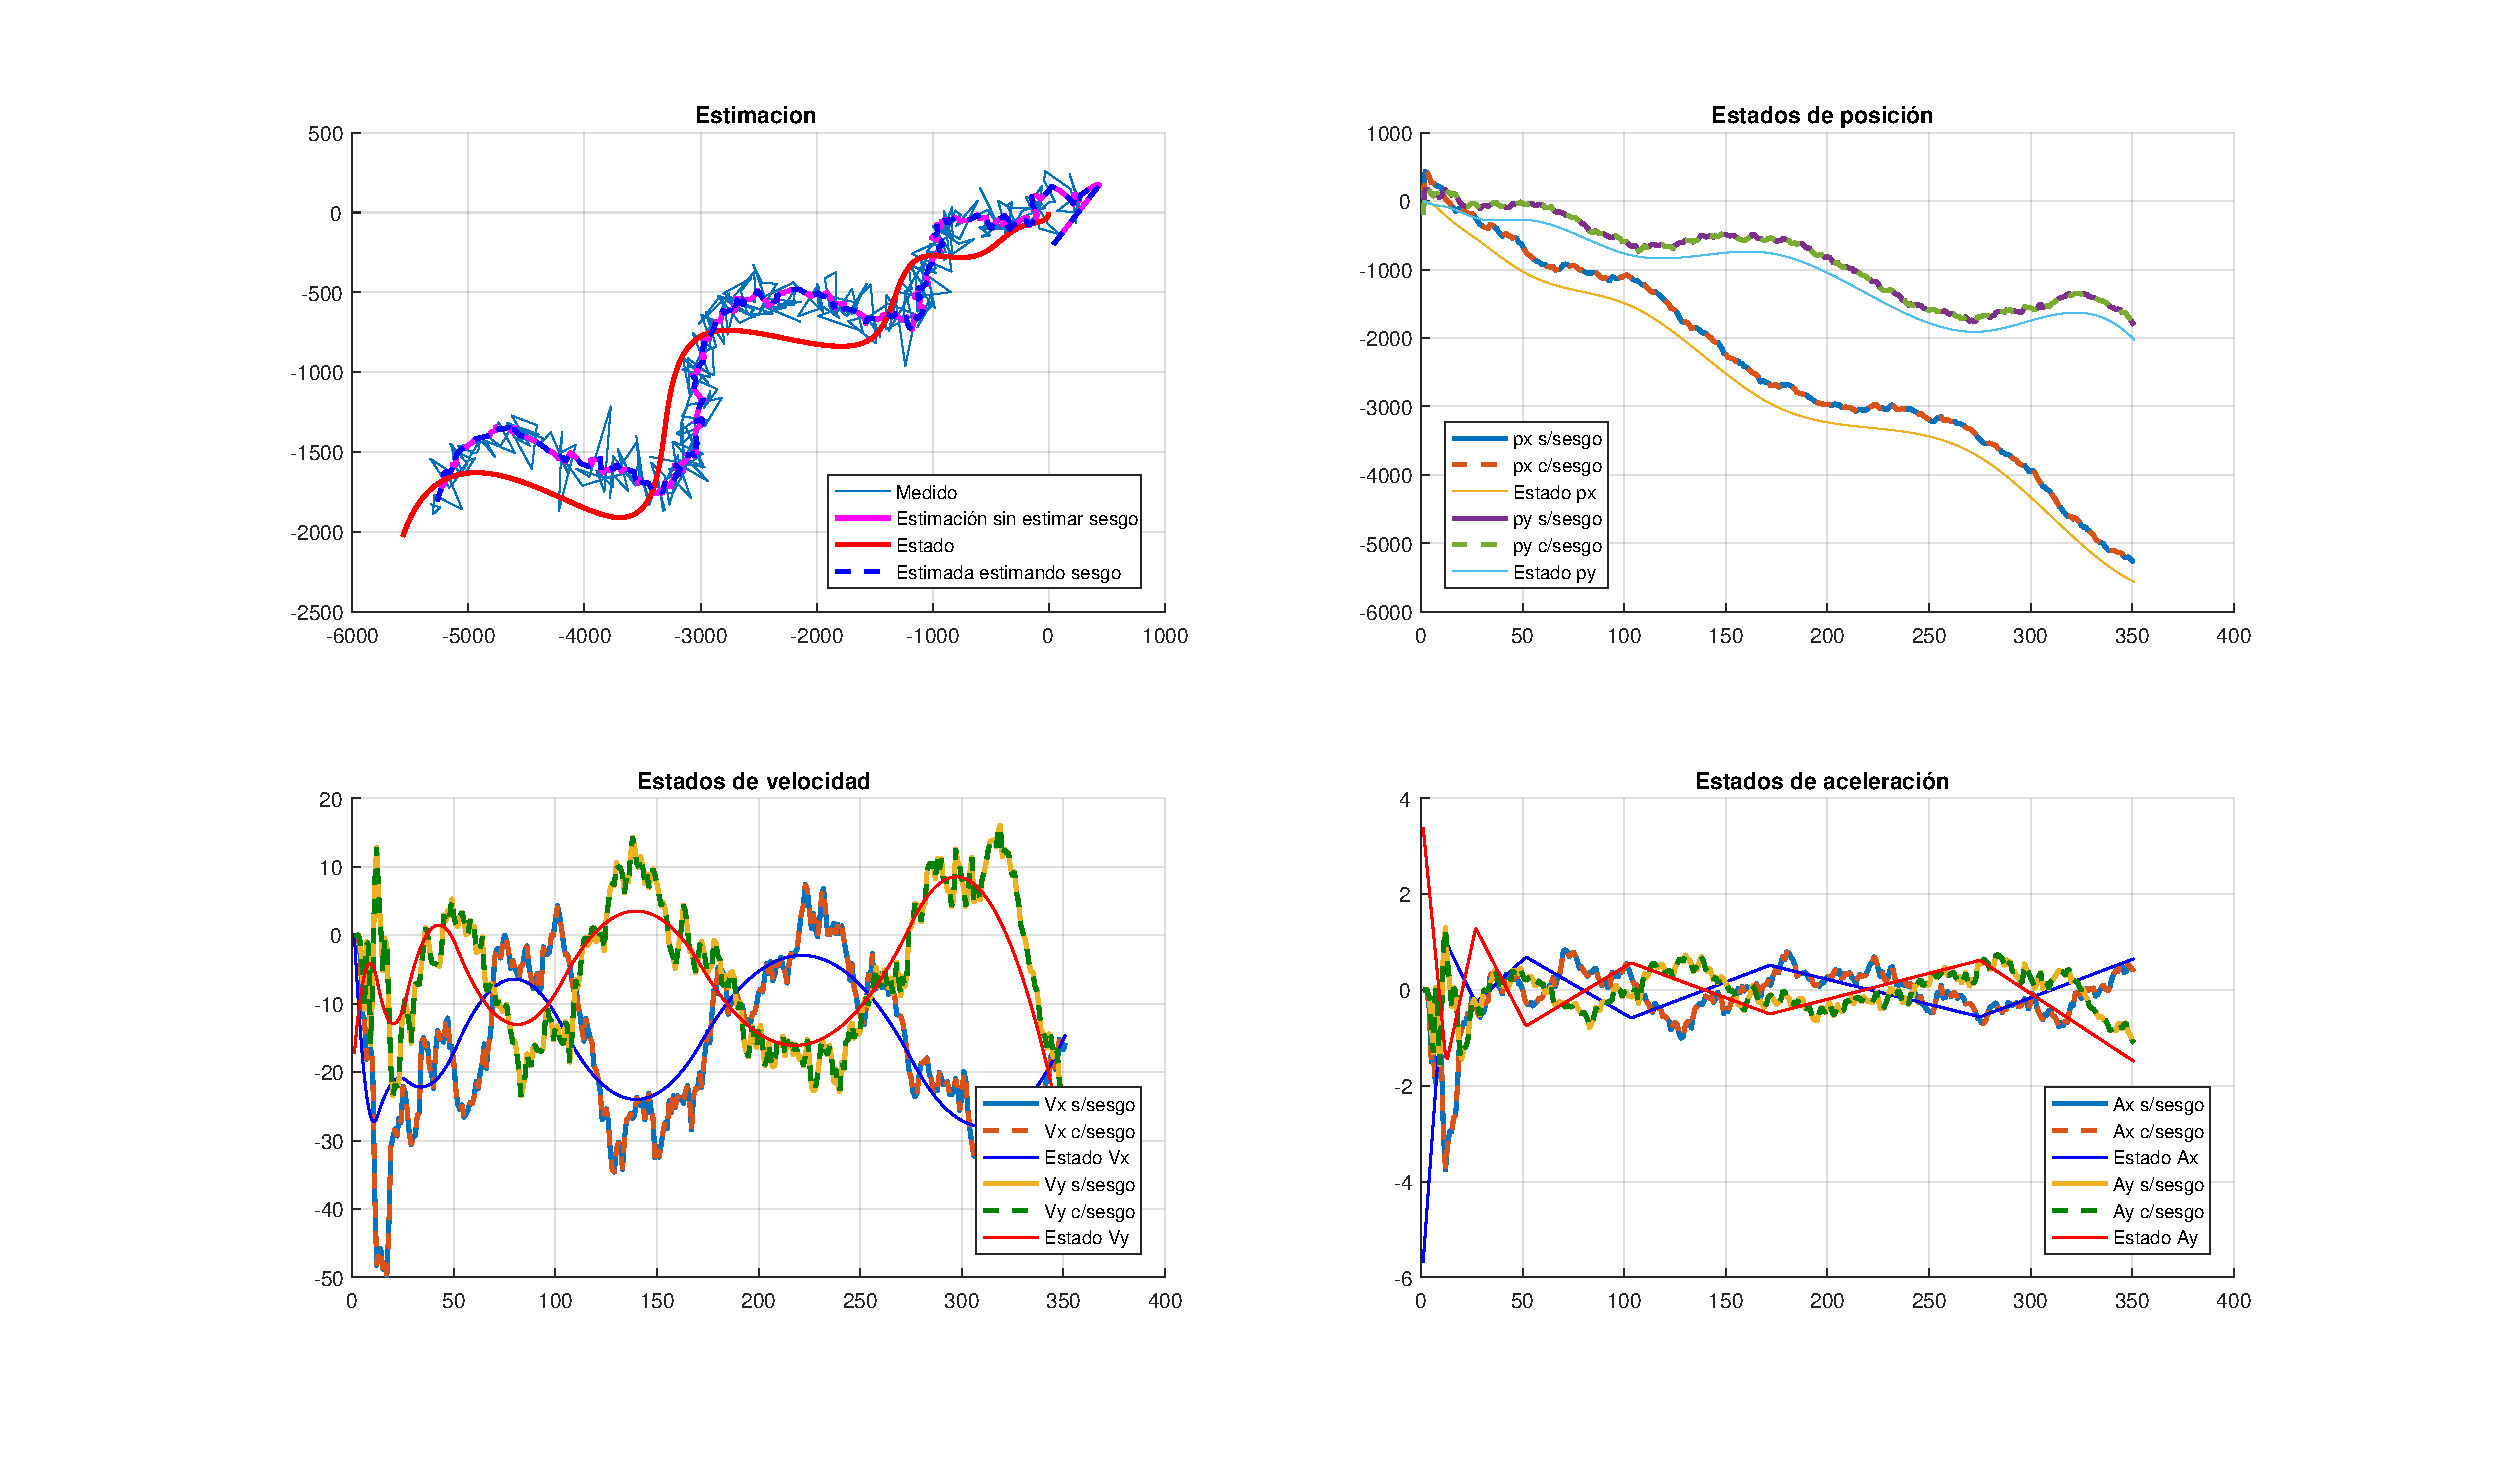
\includegraphics[width=1.0\textwidth,keepaspectratio]{Figuras/graf_ej4a.pdf}
		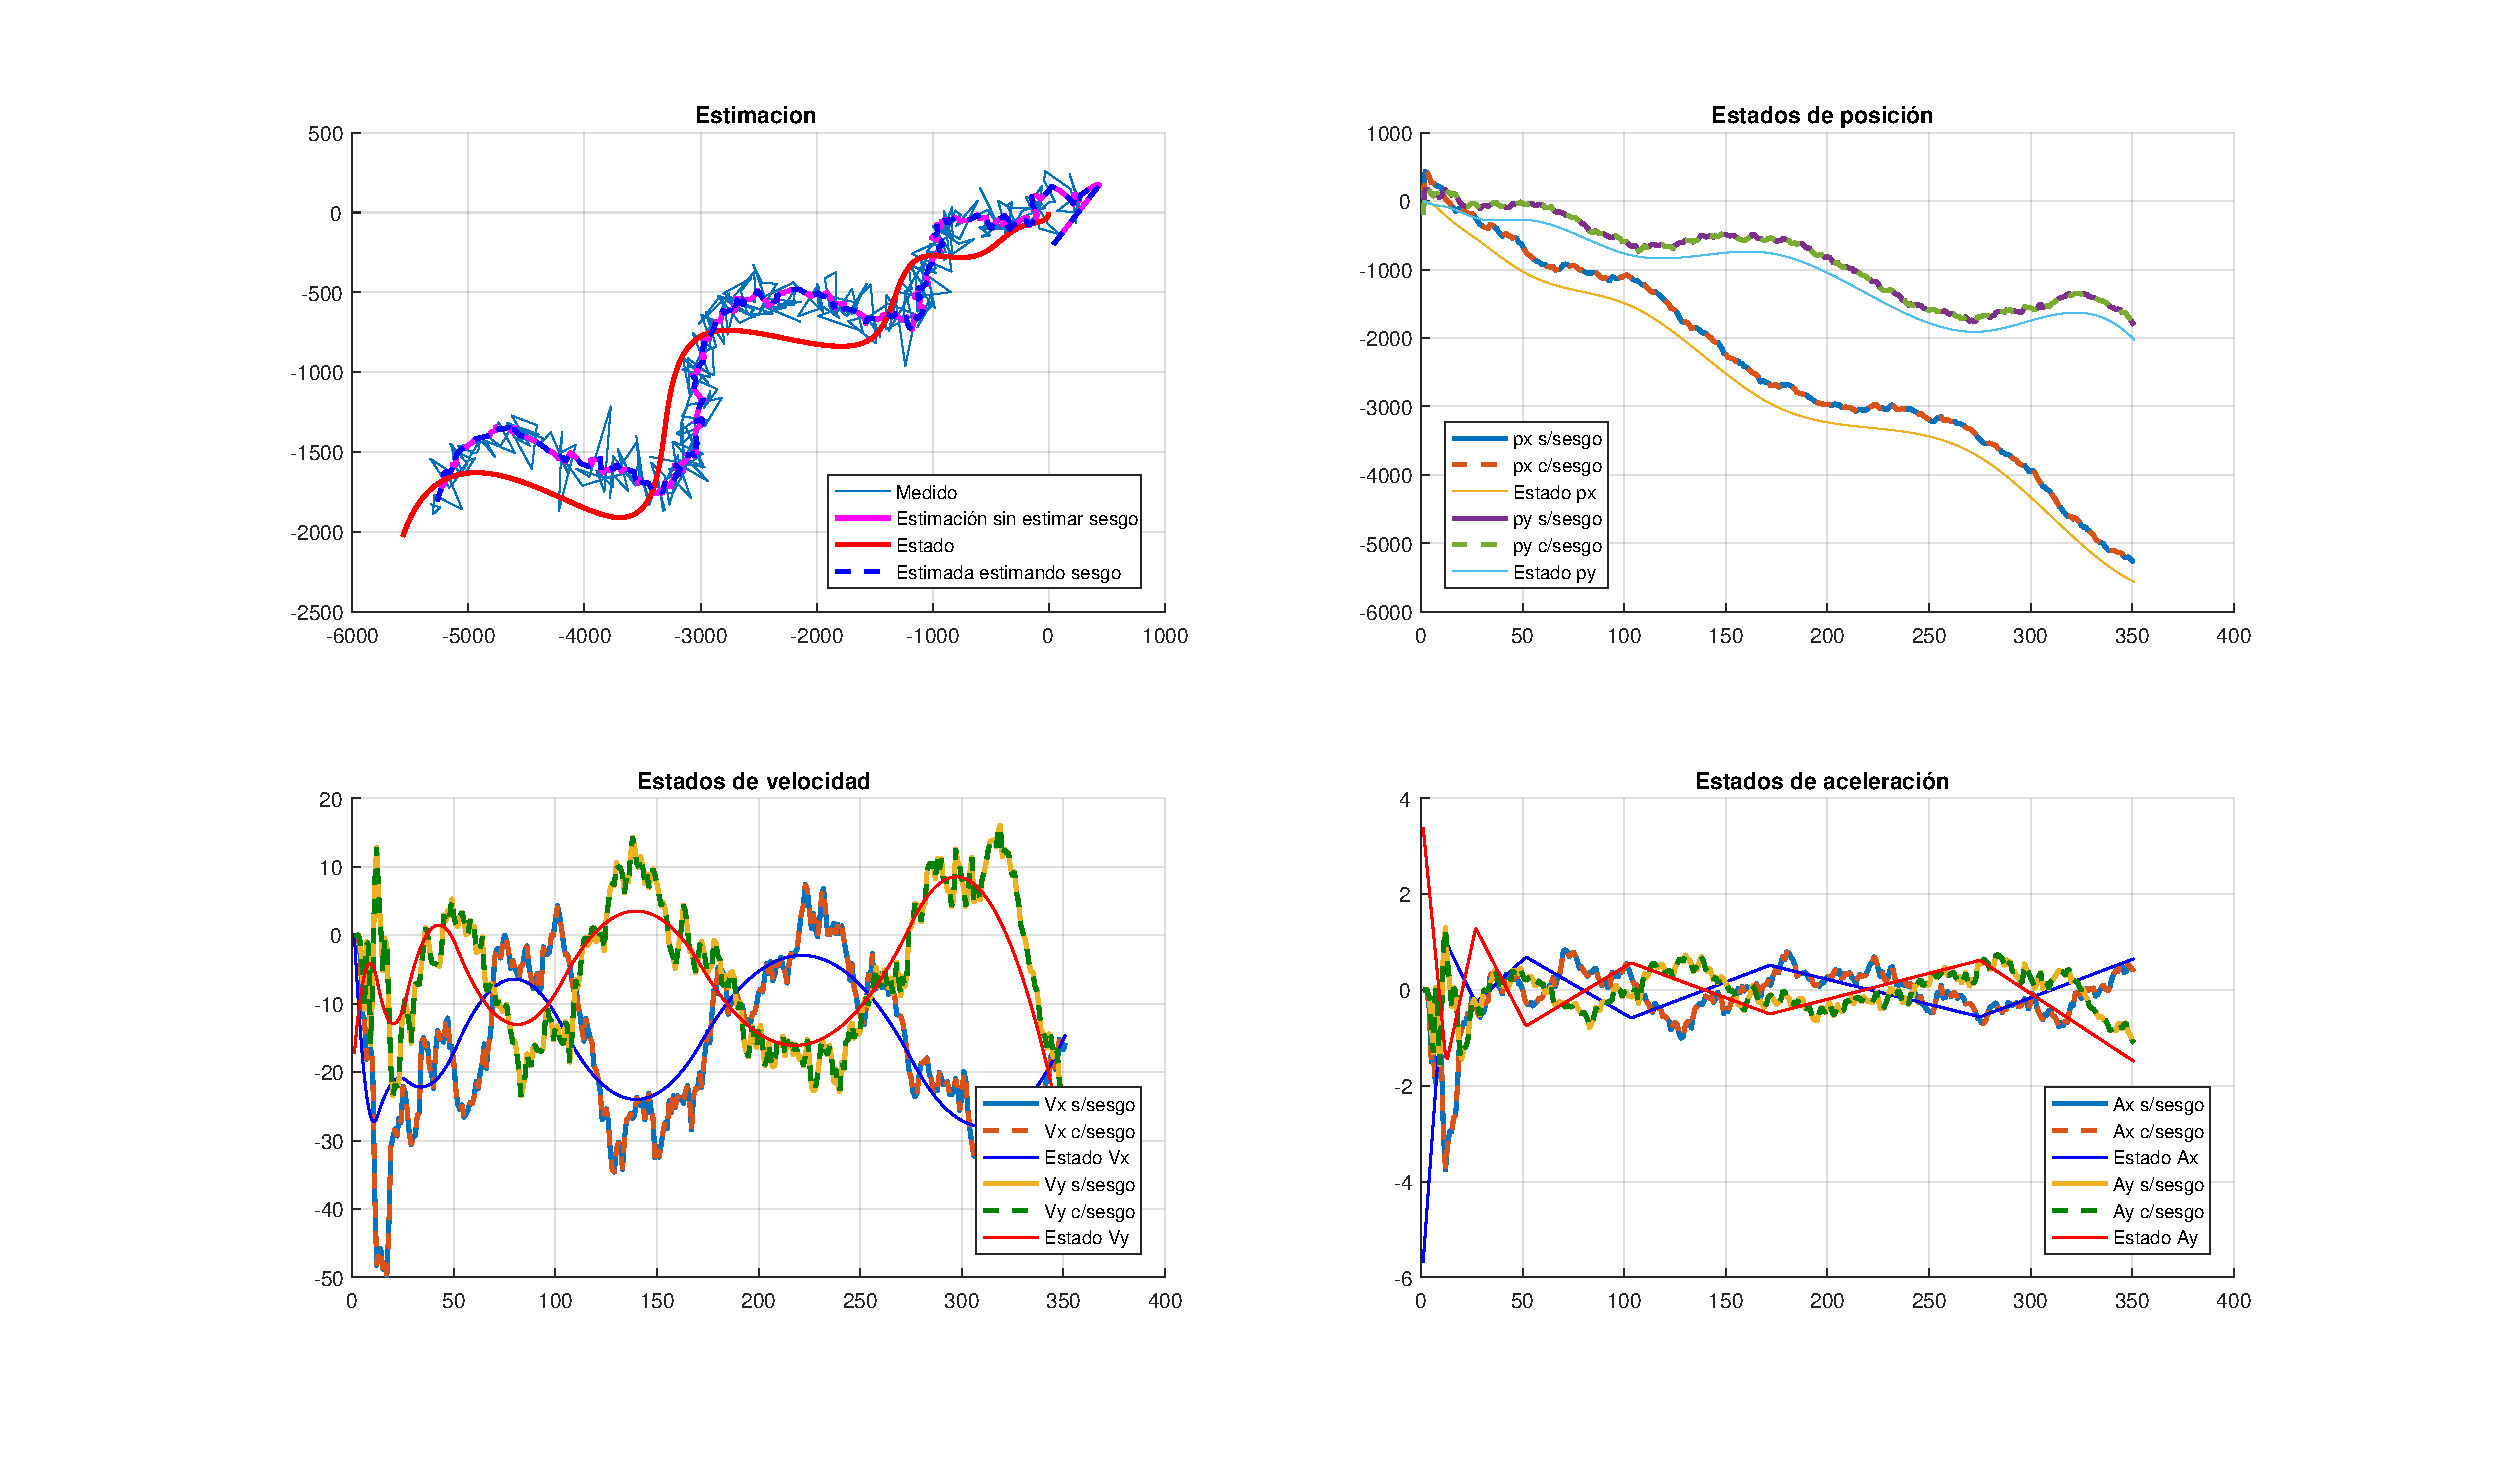
\includegraphics[scale=0.5,trim={6,5cm 0 0 0}]{Figuras/graf_ej4a.pdf}
		\caption{Estimación De Trayectoria}
		\label{fig:ej4a}
	\end{figure}
	
	En la figura \ref{fig:ej4a_bias} se observa la convergencia de la estimación del sesgo. Es posible ver que no converge exactamente al valor deseado.
	
	\begin{figure}[H]
		\centering
		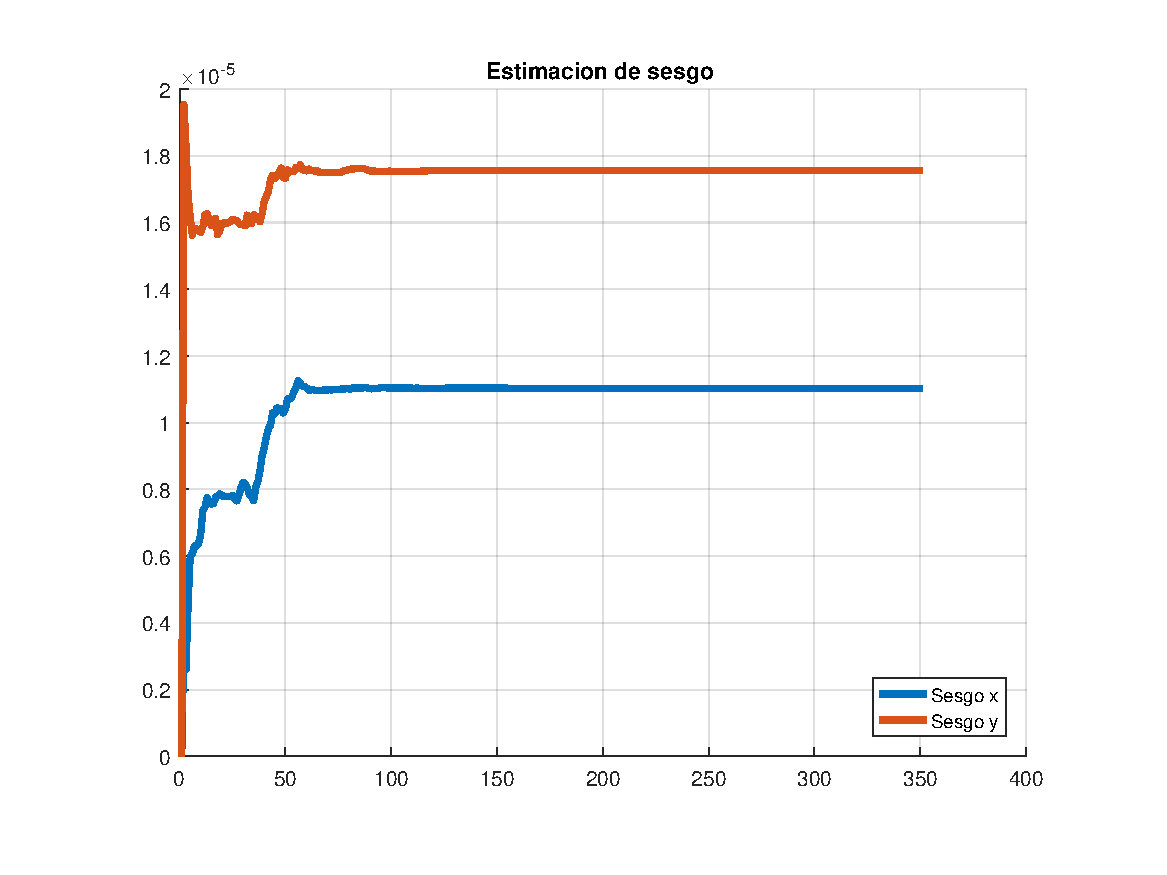
\includegraphics[width=0.7\textwidth,keepaspectratio]{Figuras/bias_ej4a.pdf}
		\caption{Estimación Del Sesgo}
		\label{fig:ej4a_bias}
	\end{figure}
	
	En la figura \ref{fig:ej4a_cov} se observa la autocorrelación de las innovaciónes. Es posible ver que se trata de un proceso blanco.
	
	\begin{figure}[H]
		\centering
		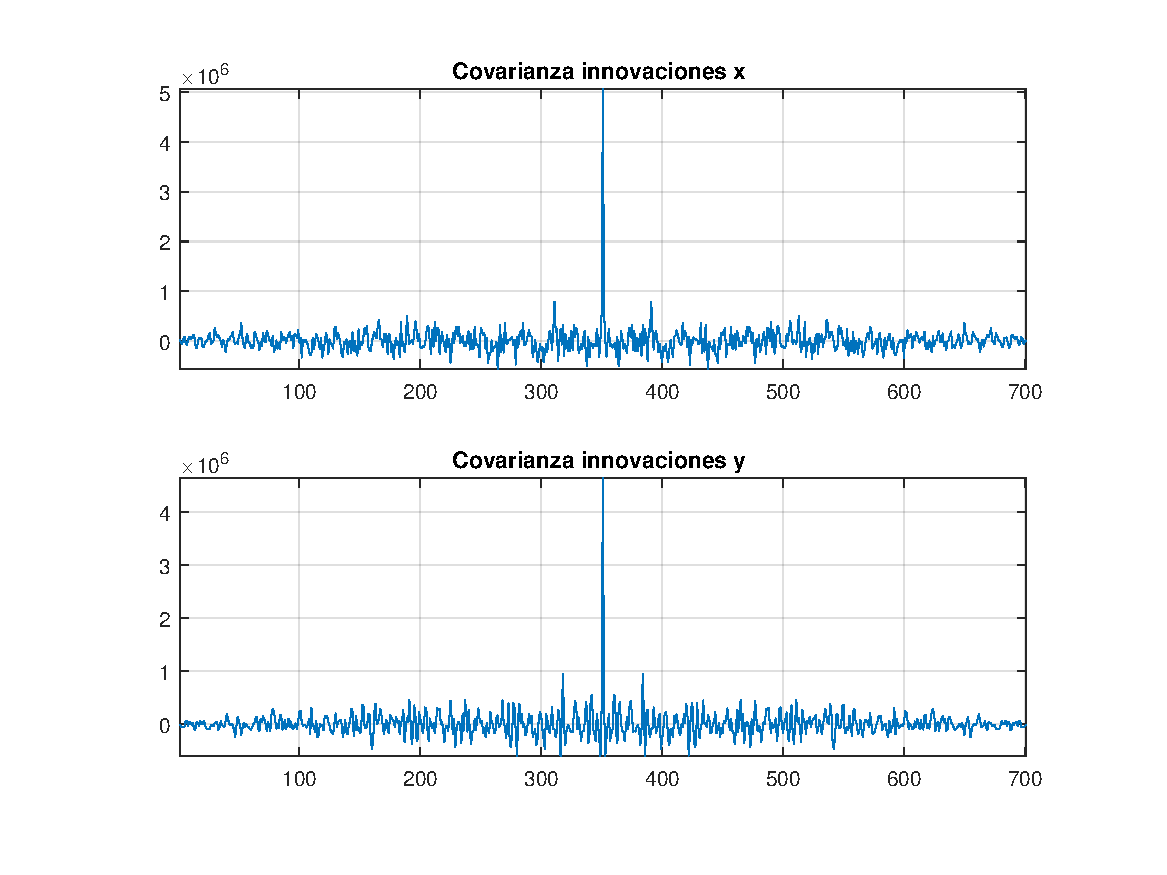
\includegraphics[width=1.0\textwidth,keepaspectratio]{Figuras/covinn_ej4a.pdf}
		\caption{Correlación De Innovaciones}
		\label{fig:ej4a_cov}
	\end{figure}
	
%--------------------------------------------------------------------------------------------------

\subsection{Medición de PVA - Sesgo en P}

	En la figura \ref{fig:ej4b} se observa el resultado de la estimación de la trayectoria. Resulta similar al caso anterior en cuanto a que funciona mejor que suponer un sesgo nulo, sin embargo el seguimiento de la trayectoria no es perfecto, problema nuevamente ligado a la observabilidad.

	\begin{figure}[H]
		\centering
		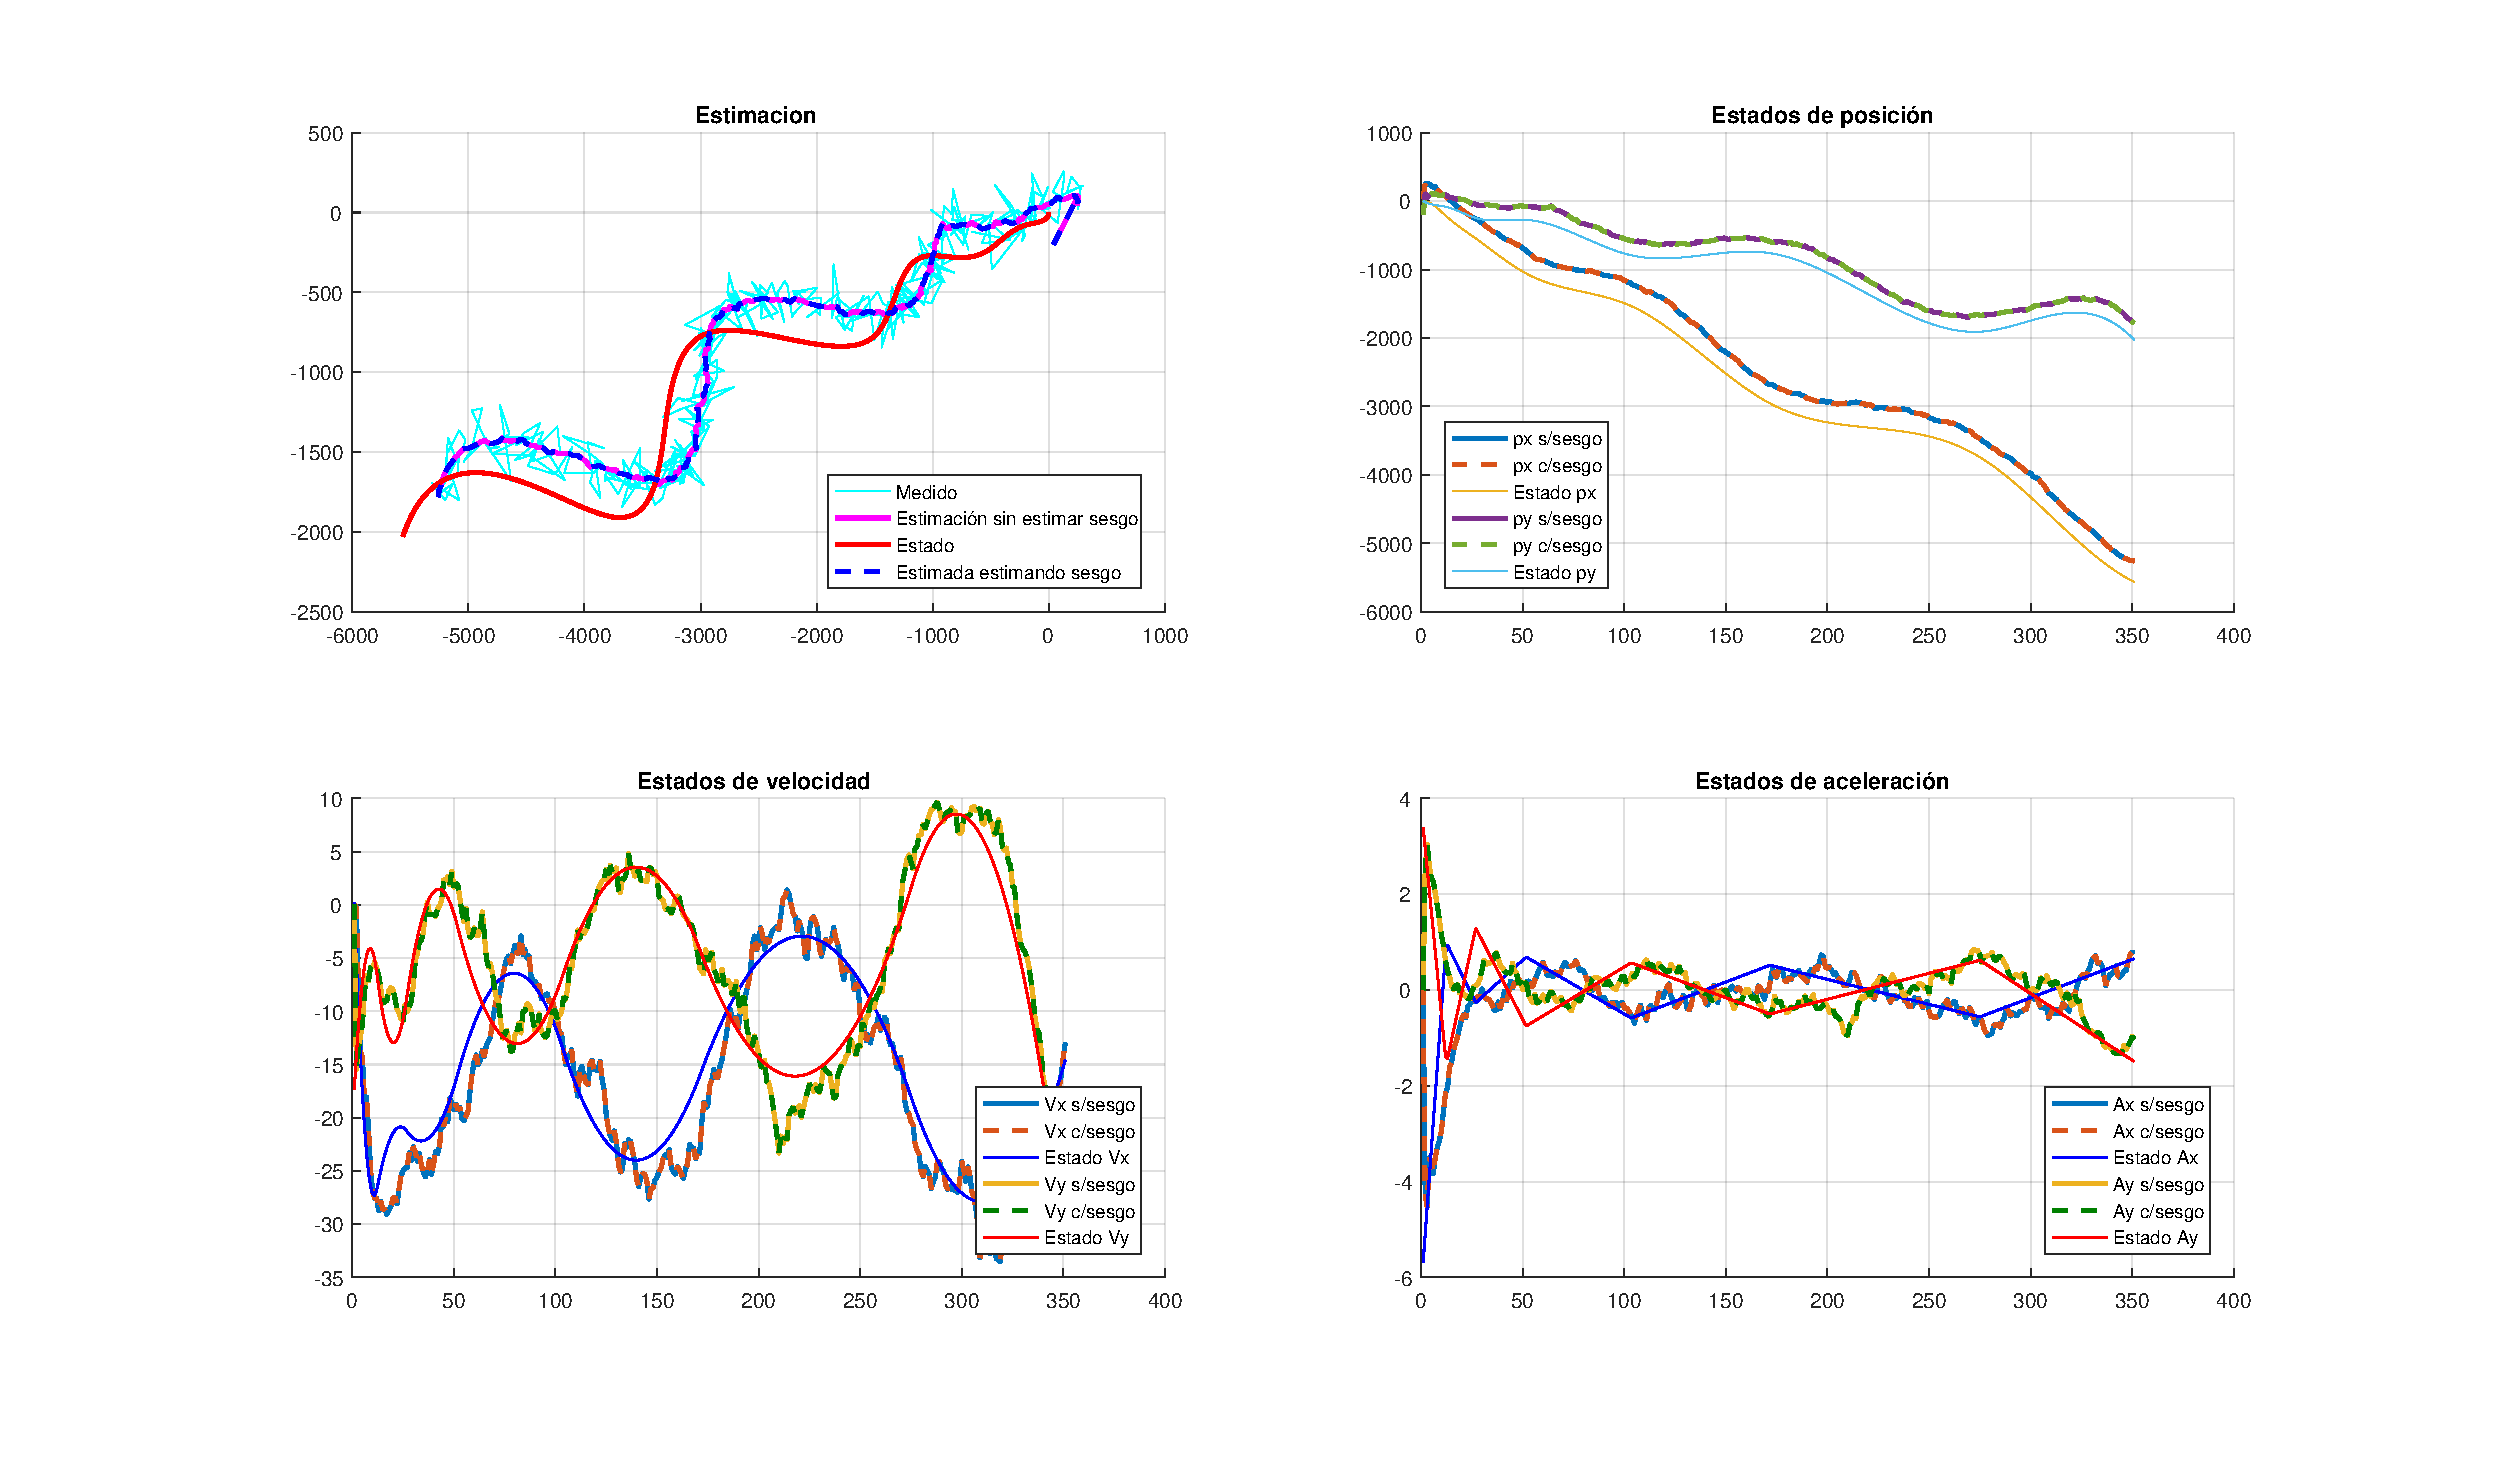
\includegraphics[scale=0.5,trim={6,5cm 0 0 0}]{Figuras/graf_ej4b.pdf}
		\caption{Estimación De Trayectoria}
		\label{fig:ej4b}
	\end{figure}
	
	En la figura \ref{fig:ej4a_bias} se observa la convergencia de la estimación del sesgo. Es posible ver que no converge exactamente al valor deseado.
	
	\begin{figure}[H]
		\centering
		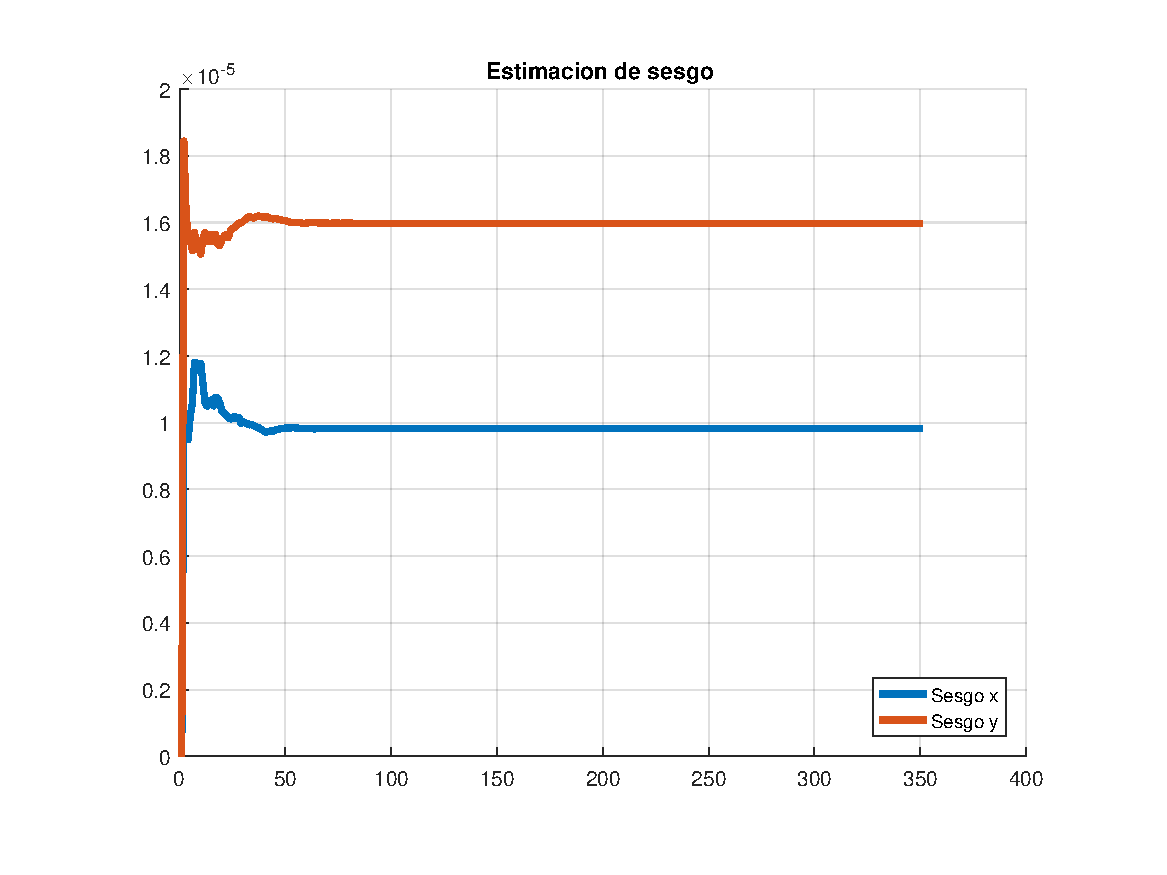
\includegraphics[width=0.7\textwidth,keepaspectratio]{Figuras/bias_ej4b.pdf}
		\caption{Estimación Del Sesgo}
		\label{fig:ej4b_bias}
	\end{figure}
	
	En la figura \ref{fig:ej4a_cov} se observa la autocorrelación de las innovaciónes. Es posible ver que se trata de un proceso blanco.
	
	\begin{figure}[H]
		\centering
		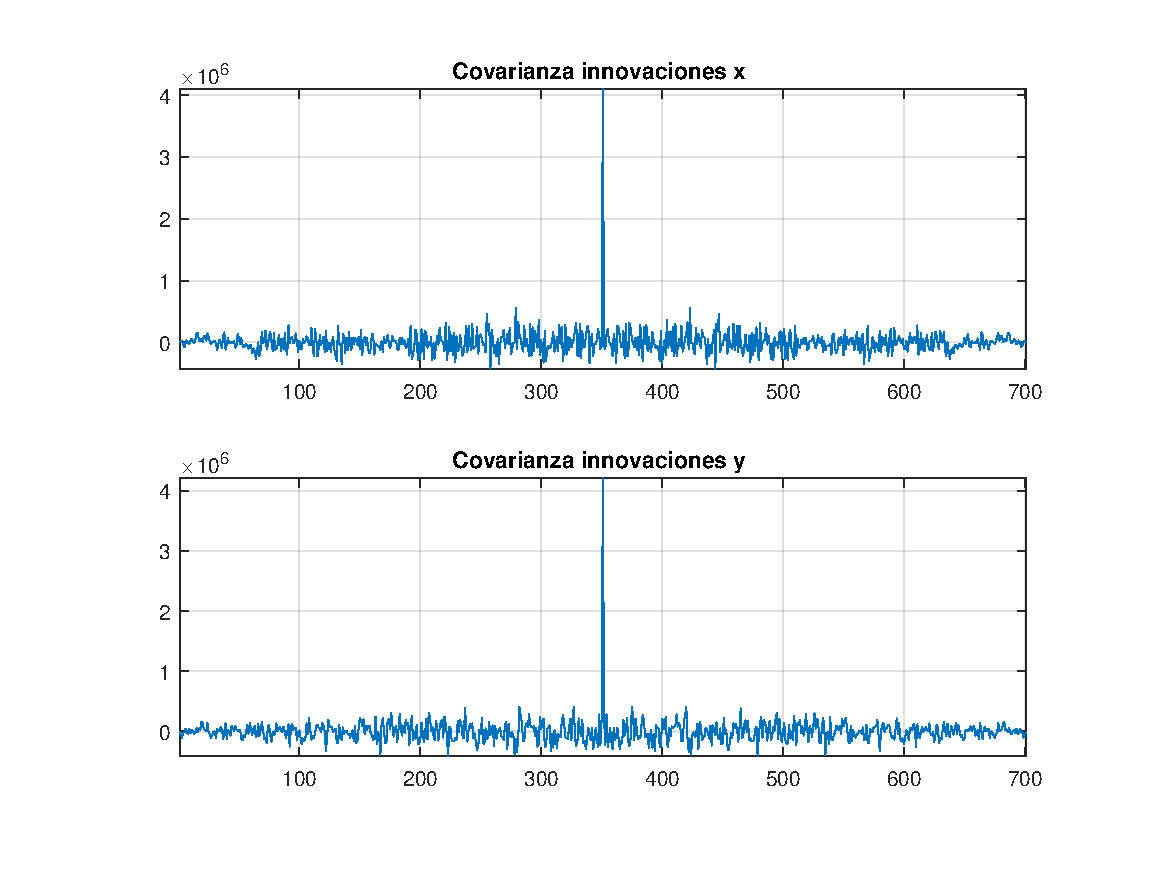
\includegraphics[width=1.0\textwidth,keepaspectratio]{Figuras/covinn_ej4b.pdf}
		\caption{Correlación De Innovaciones}
		\label{fig:ej4b_cov}
	\end{figure}
	
%--------------------------------------------------------------------------------------------------
	
\subsection{Medición de V - Sesgo en V}

	En la figura \ref{fig:ej4c} se observa el resultado de la estimación. En la misma la estimación no sólo no sigue la trayectoria, sino que se aparta cada vez más de ella a medida que transcurre el tiempo, tanto si se ignora el sesgo, como si se trata de estimarlo (Problemas de observabilidad).

	\begin{figure}[H]
		\centering
		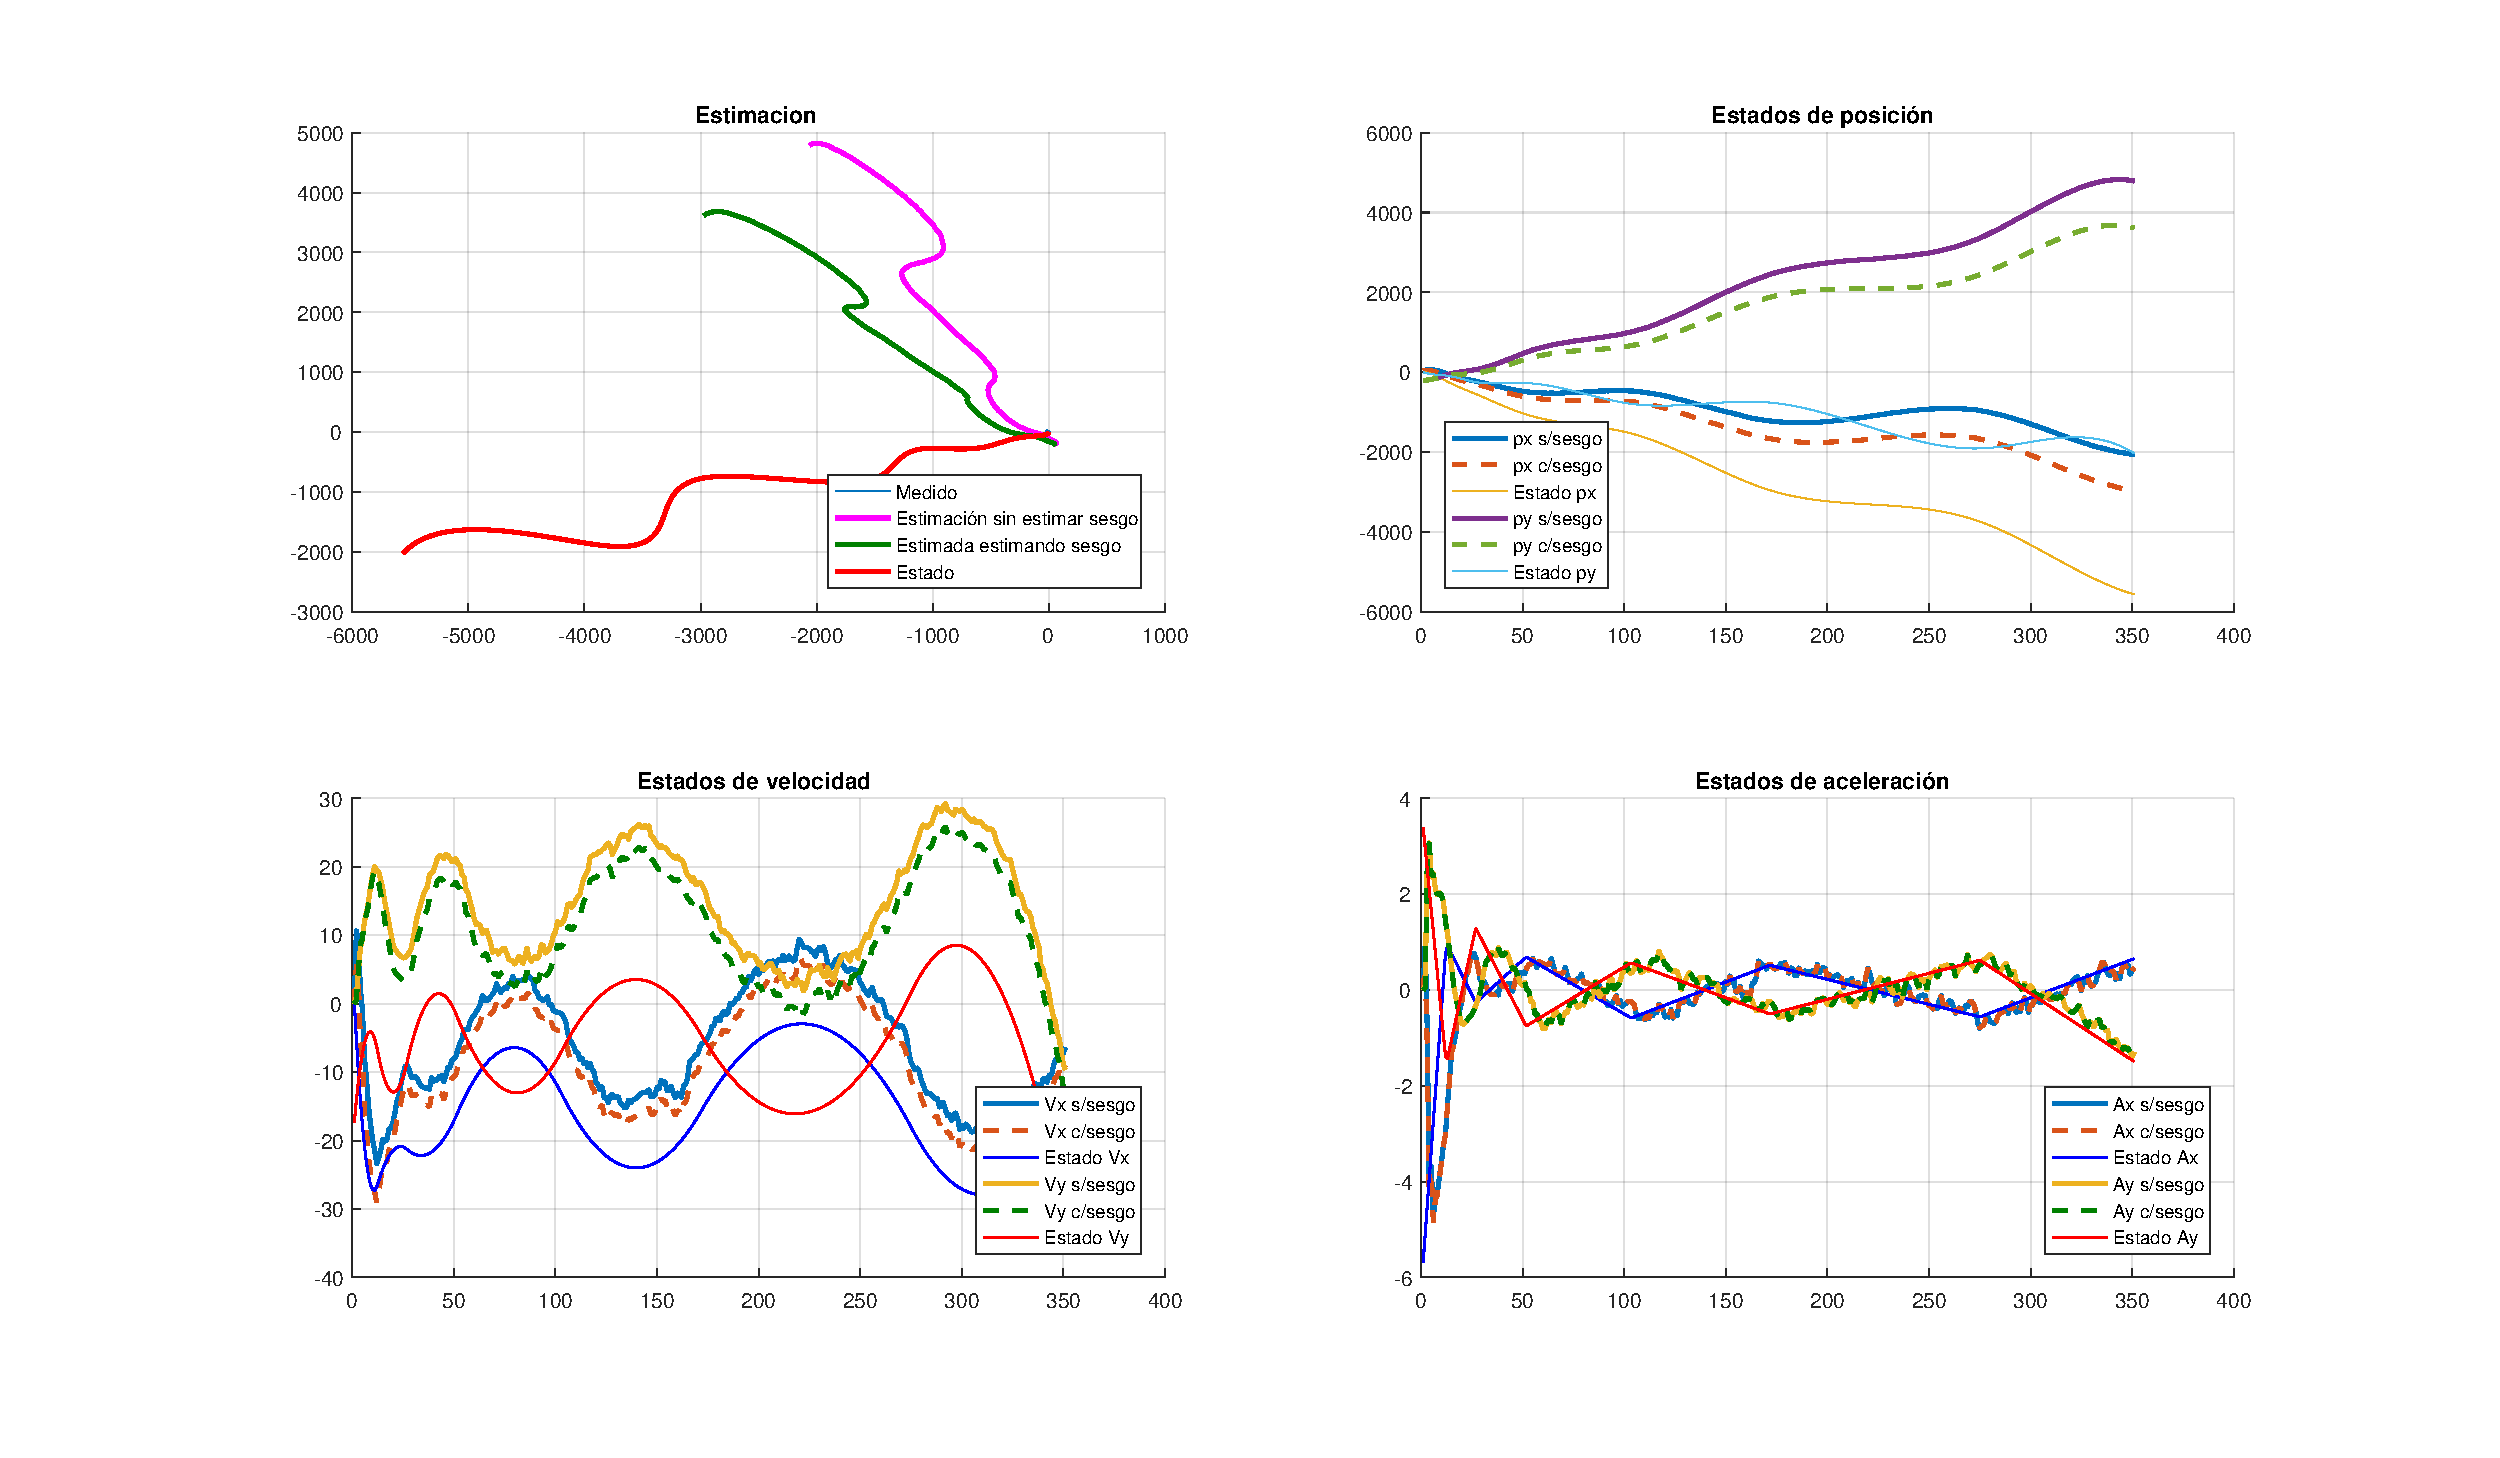
\includegraphics[scale=0.5,trim={6,5cm 0 0 0}]{Figuras/graf_ej4c.pdf}
		\caption{Estimación De Trayectoria}
		\label{fig:ej4c}
	\end{figure}
	
	En la figura \ref{fig:ej4c_bias} se observa que la estimación converge, pero no a los valores correctos.
	
	\begin{figure}[H]
		\centering
		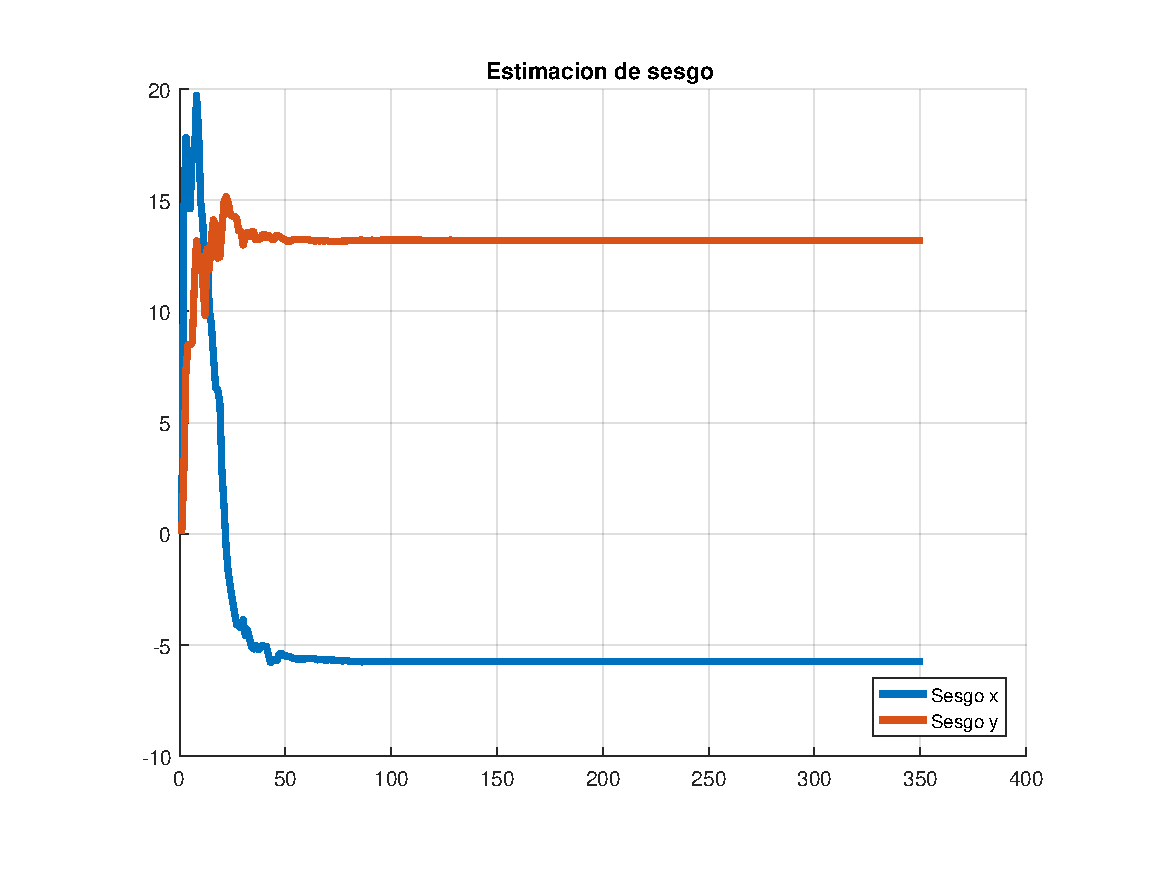
\includegraphics[width=0.7\textwidth,keepaspectratio]{Figuras/bias_ej4c.pdf}
		\caption{Estimación Del Sesgo}
		\label{fig:ej4c_bias}
	\end{figure}
	
	En la figura \ref{fig:ej4c_cov} se observa la autocorrelación innovaciónes. Es posible ver que el proceso ya no es del todo blanco.
	
	\begin{figure}[H]
		\centering
		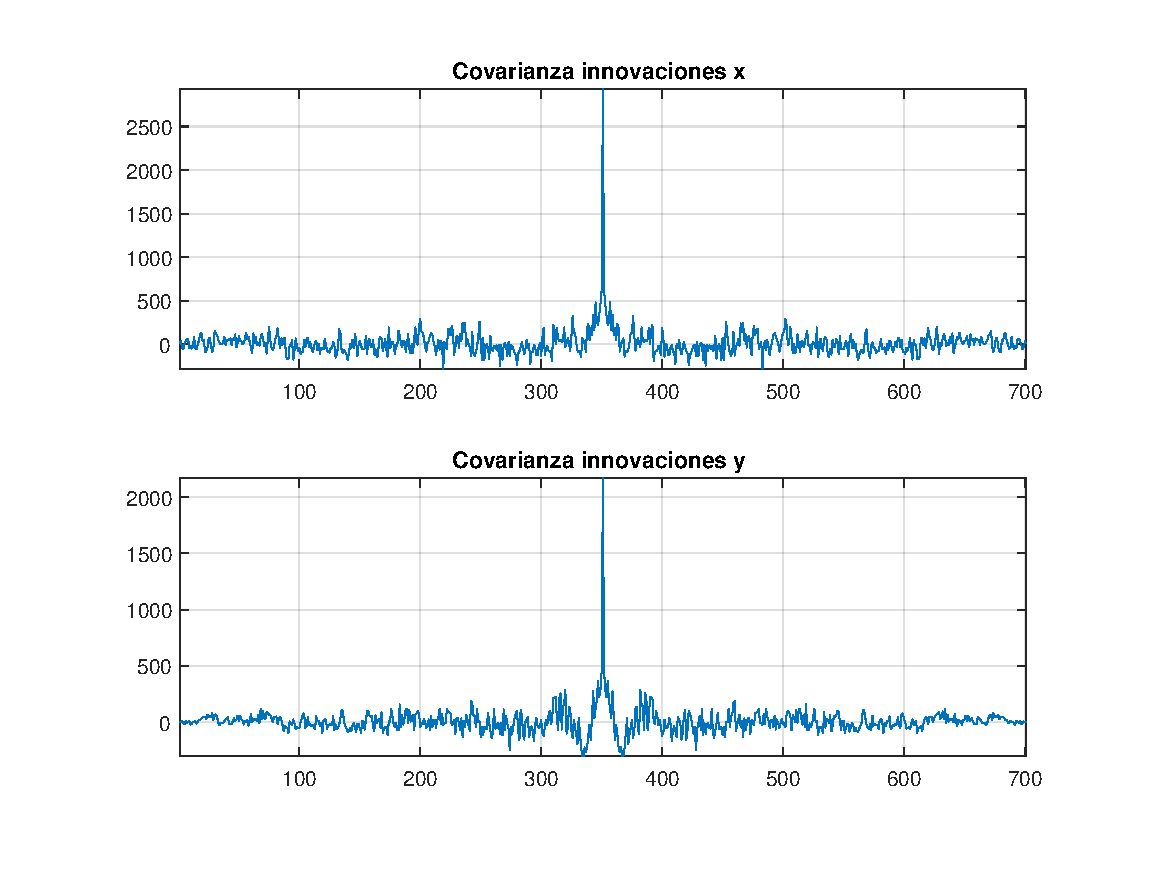
\includegraphics[width=1.0\textwidth,keepaspectratio]{Figuras/covinn_ej4c.pdf}
		\caption{Correlación De Innovaciones}
		\label{fig:ej4c_cov}
	\end{figure}
	
%--------------------------------------------------------------------------------------------------

\subsection{Medición de PVA - Sesgo en V}

	En la figura \ref{fig:ej4d} puede observarse el resultado de la estimación. En este caso no tenemos problemas de observabilidad, por lo que la estimación sigue la trayectoria y además sigue los valores de velocidad reales.

	\begin{figure}[H]
		\centering
		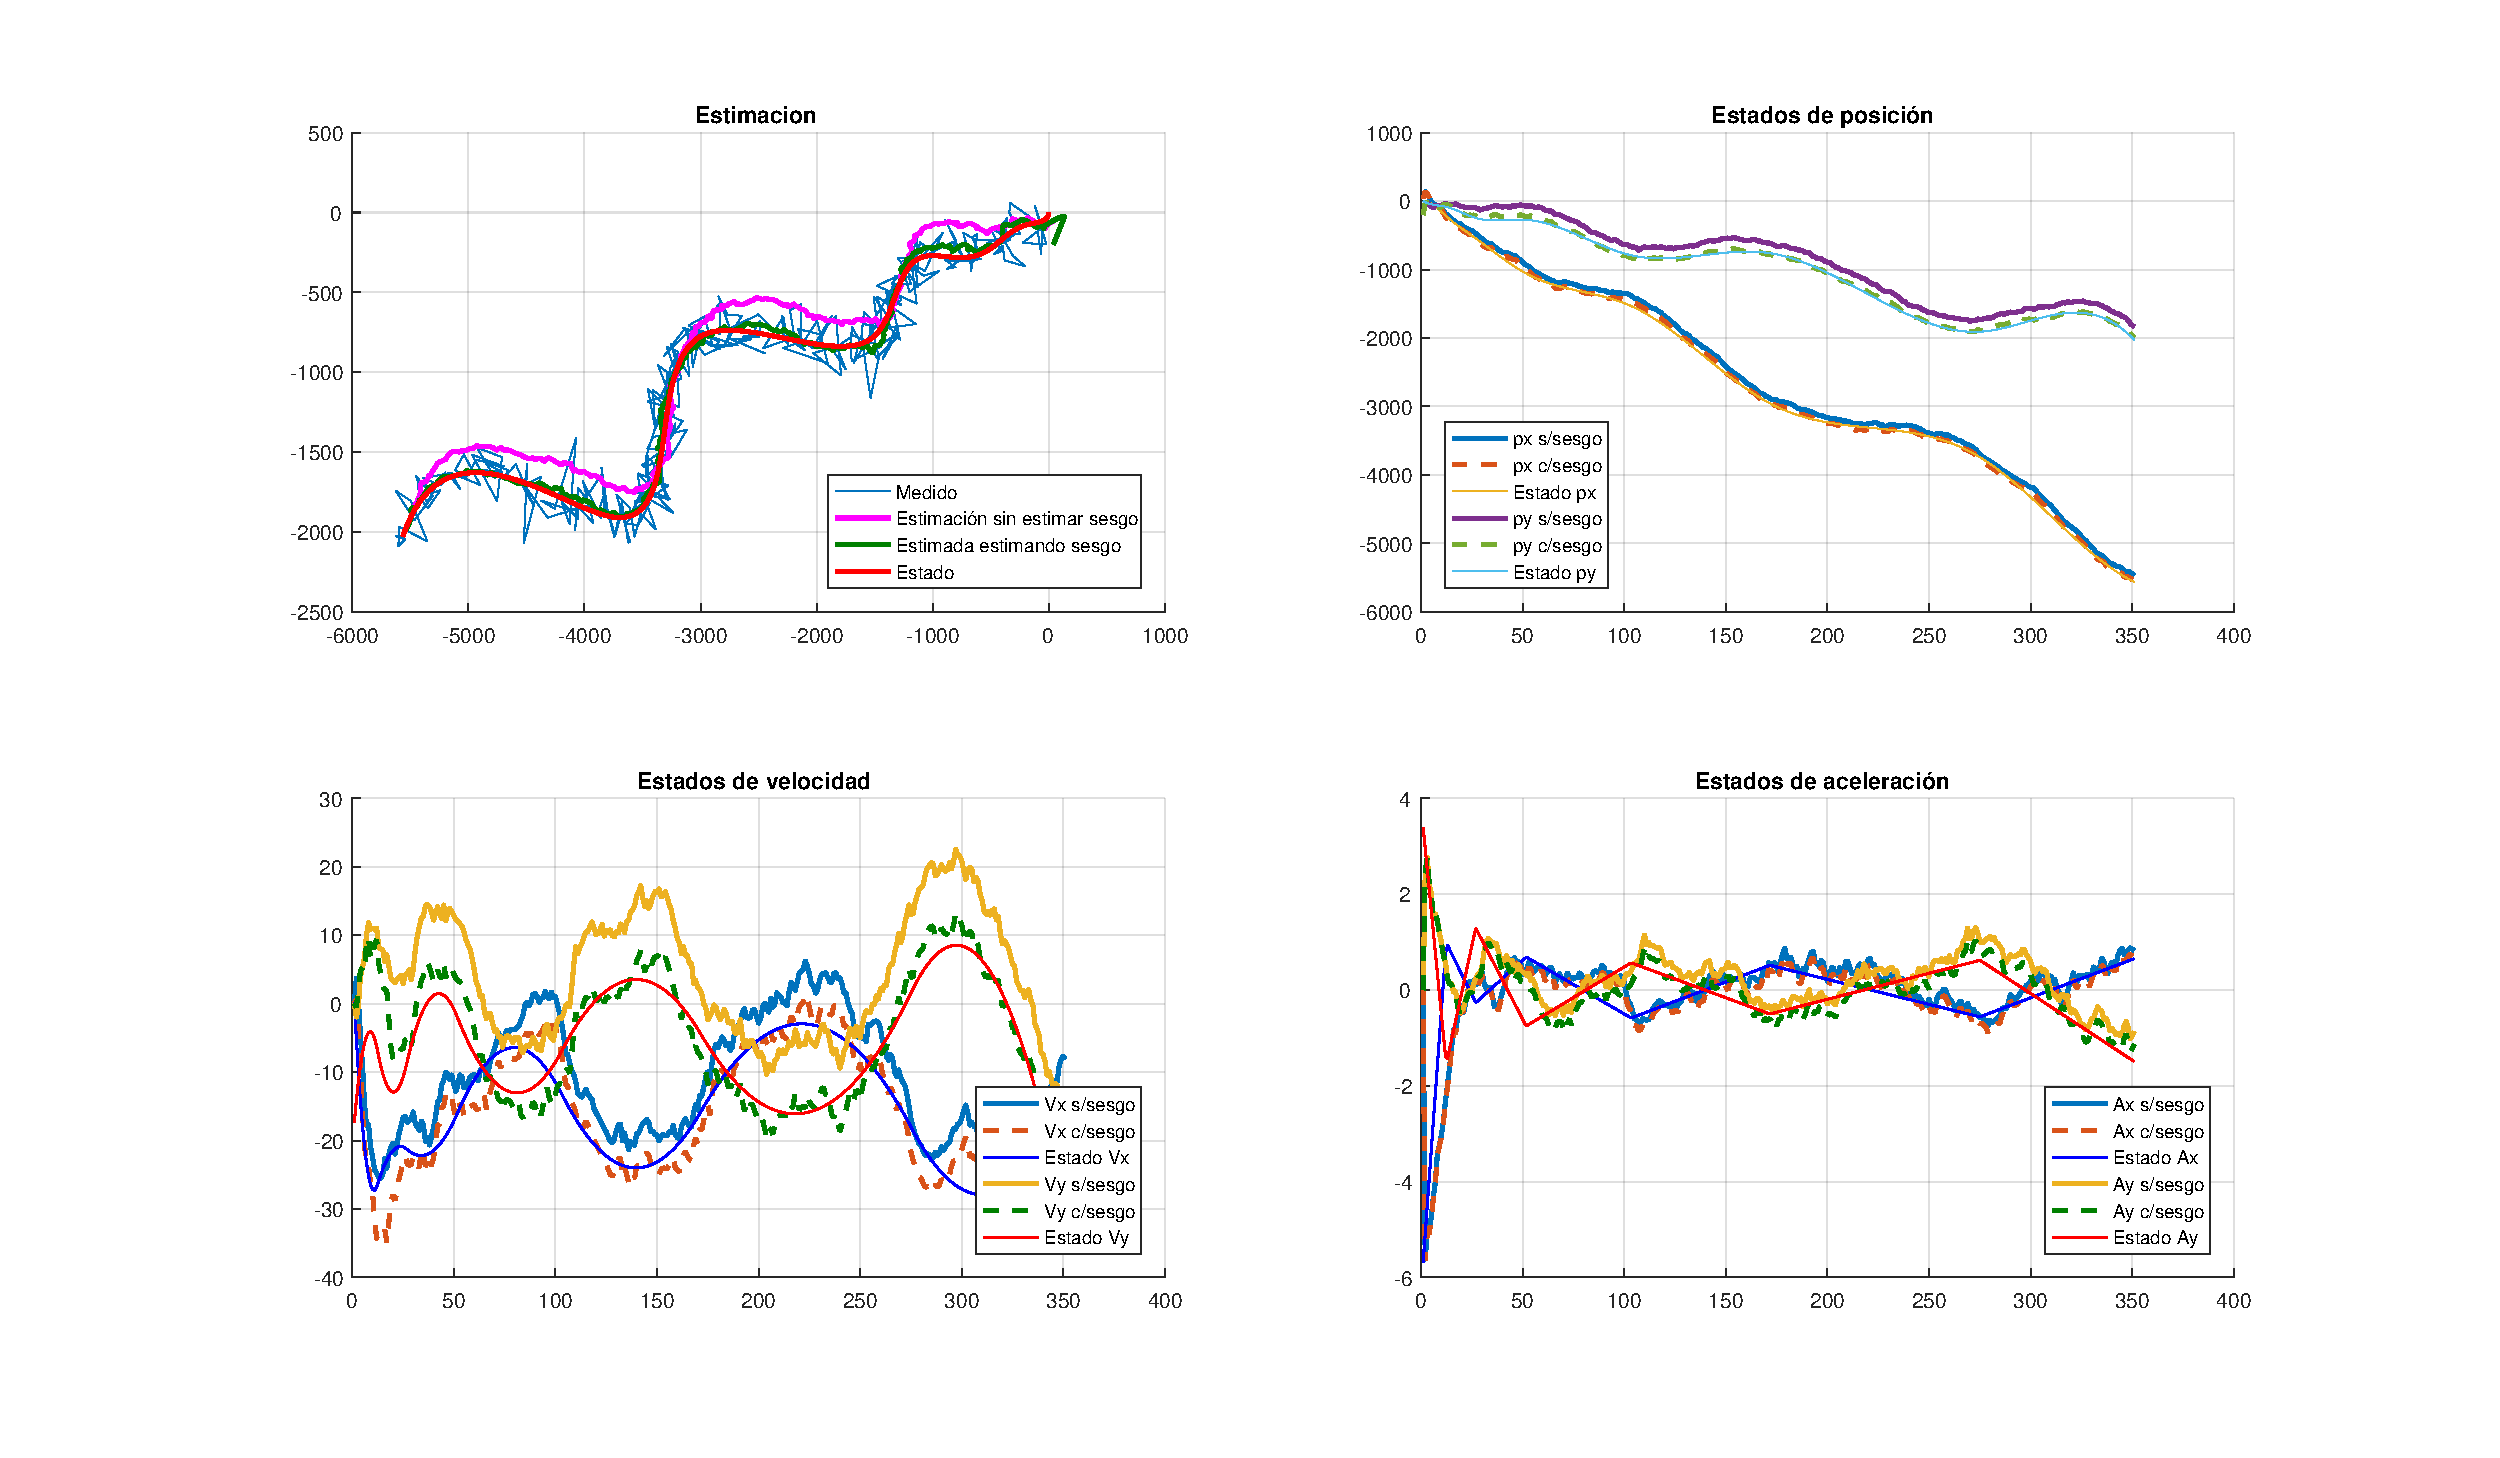
\includegraphics[scale=0.5,trim={6,5cm 0 0 0}]{Figuras/graf_ej4d.pdf}
		\caption{Estimación De Trayectoria}
		\label{fig:ej4d}
	\end{figure}
	
	En la figura \ref{fig:ej4d_bias} se observa la convergencia de la estimación del sesgo. Al no tener problemas de observabilidad, puede comprobarse que converge a los valores correctos.
	
	\begin{figure}[H]
		\centering
		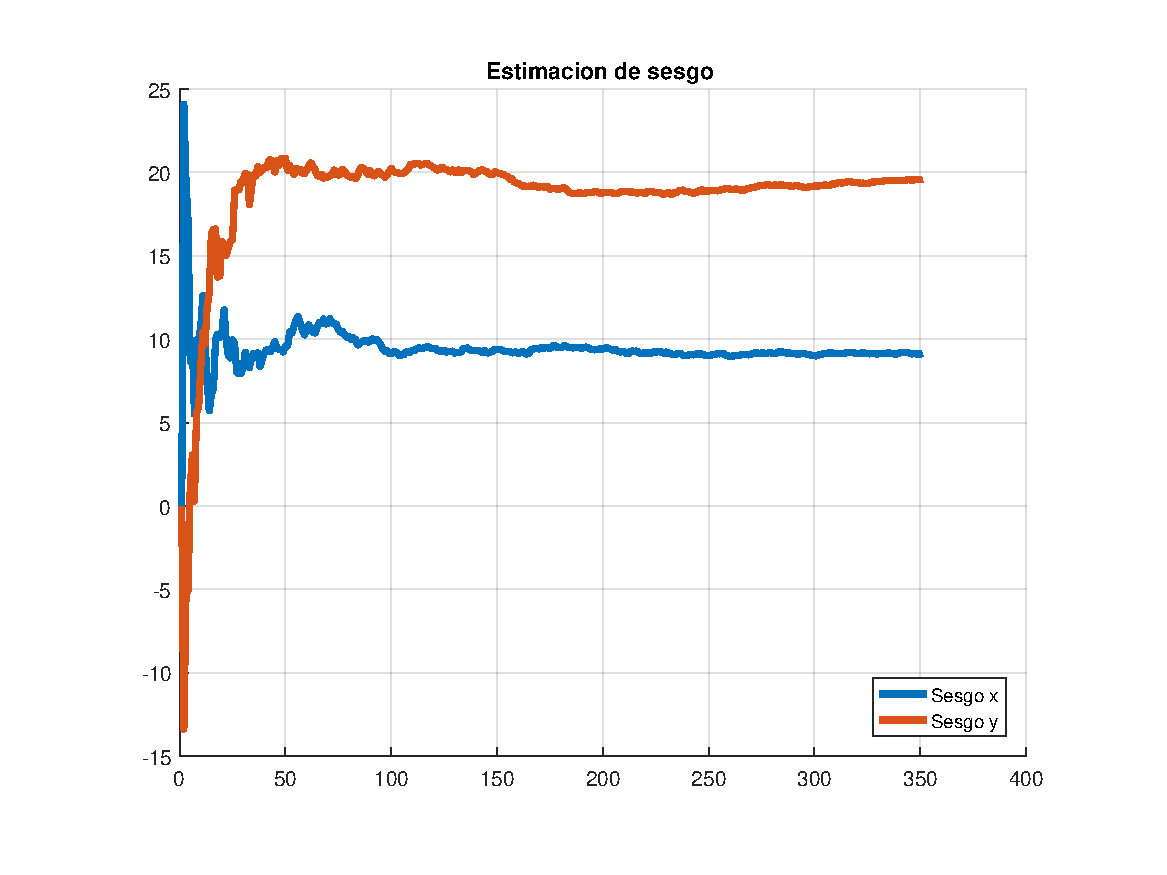
\includegraphics[width=0.7\textwidth,keepaspectratio]{Figuras/bias_ej4d.pdf}
		\caption{Estimación Del Sesgo}
		\label{fig:ej4d_bias}
	\end{figure}
	
	En la figura \ref{fig:ej4d_cov} se observa la autocorrelación de las innovaciones. Allí puede notarse que ya no es un proceso blanco.
	
	\begin{figure}[H]
		\centering
		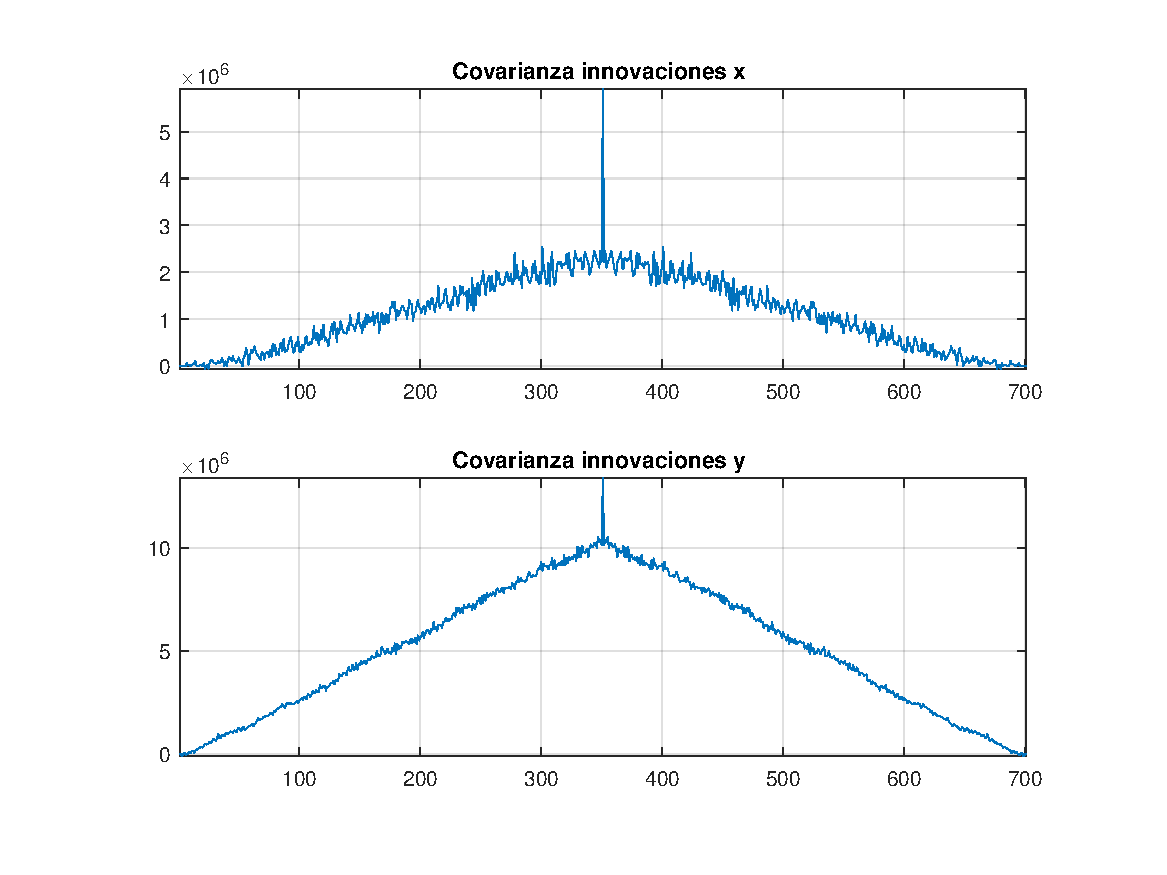
\includegraphics[width=1.0\textwidth,keepaspectratio]{Figuras/covinn_ej4d.pdf}
		\caption{Correlación De Innovaciones}
		\label{fig:ej4d_cov}
	\end{figure}

%--------------------------------------------------------------------------------------------------

\subsection{Medición de A - Sesgo en A}

	En la figura \ref{fig:ej4e} podemos observar el resultado de la estimación. En este caso no tenemos observabilidad, por lo que el resultado empeora cada vez más a medida que pasa el tiempo.

	\begin{figure}[H]
		\centering
		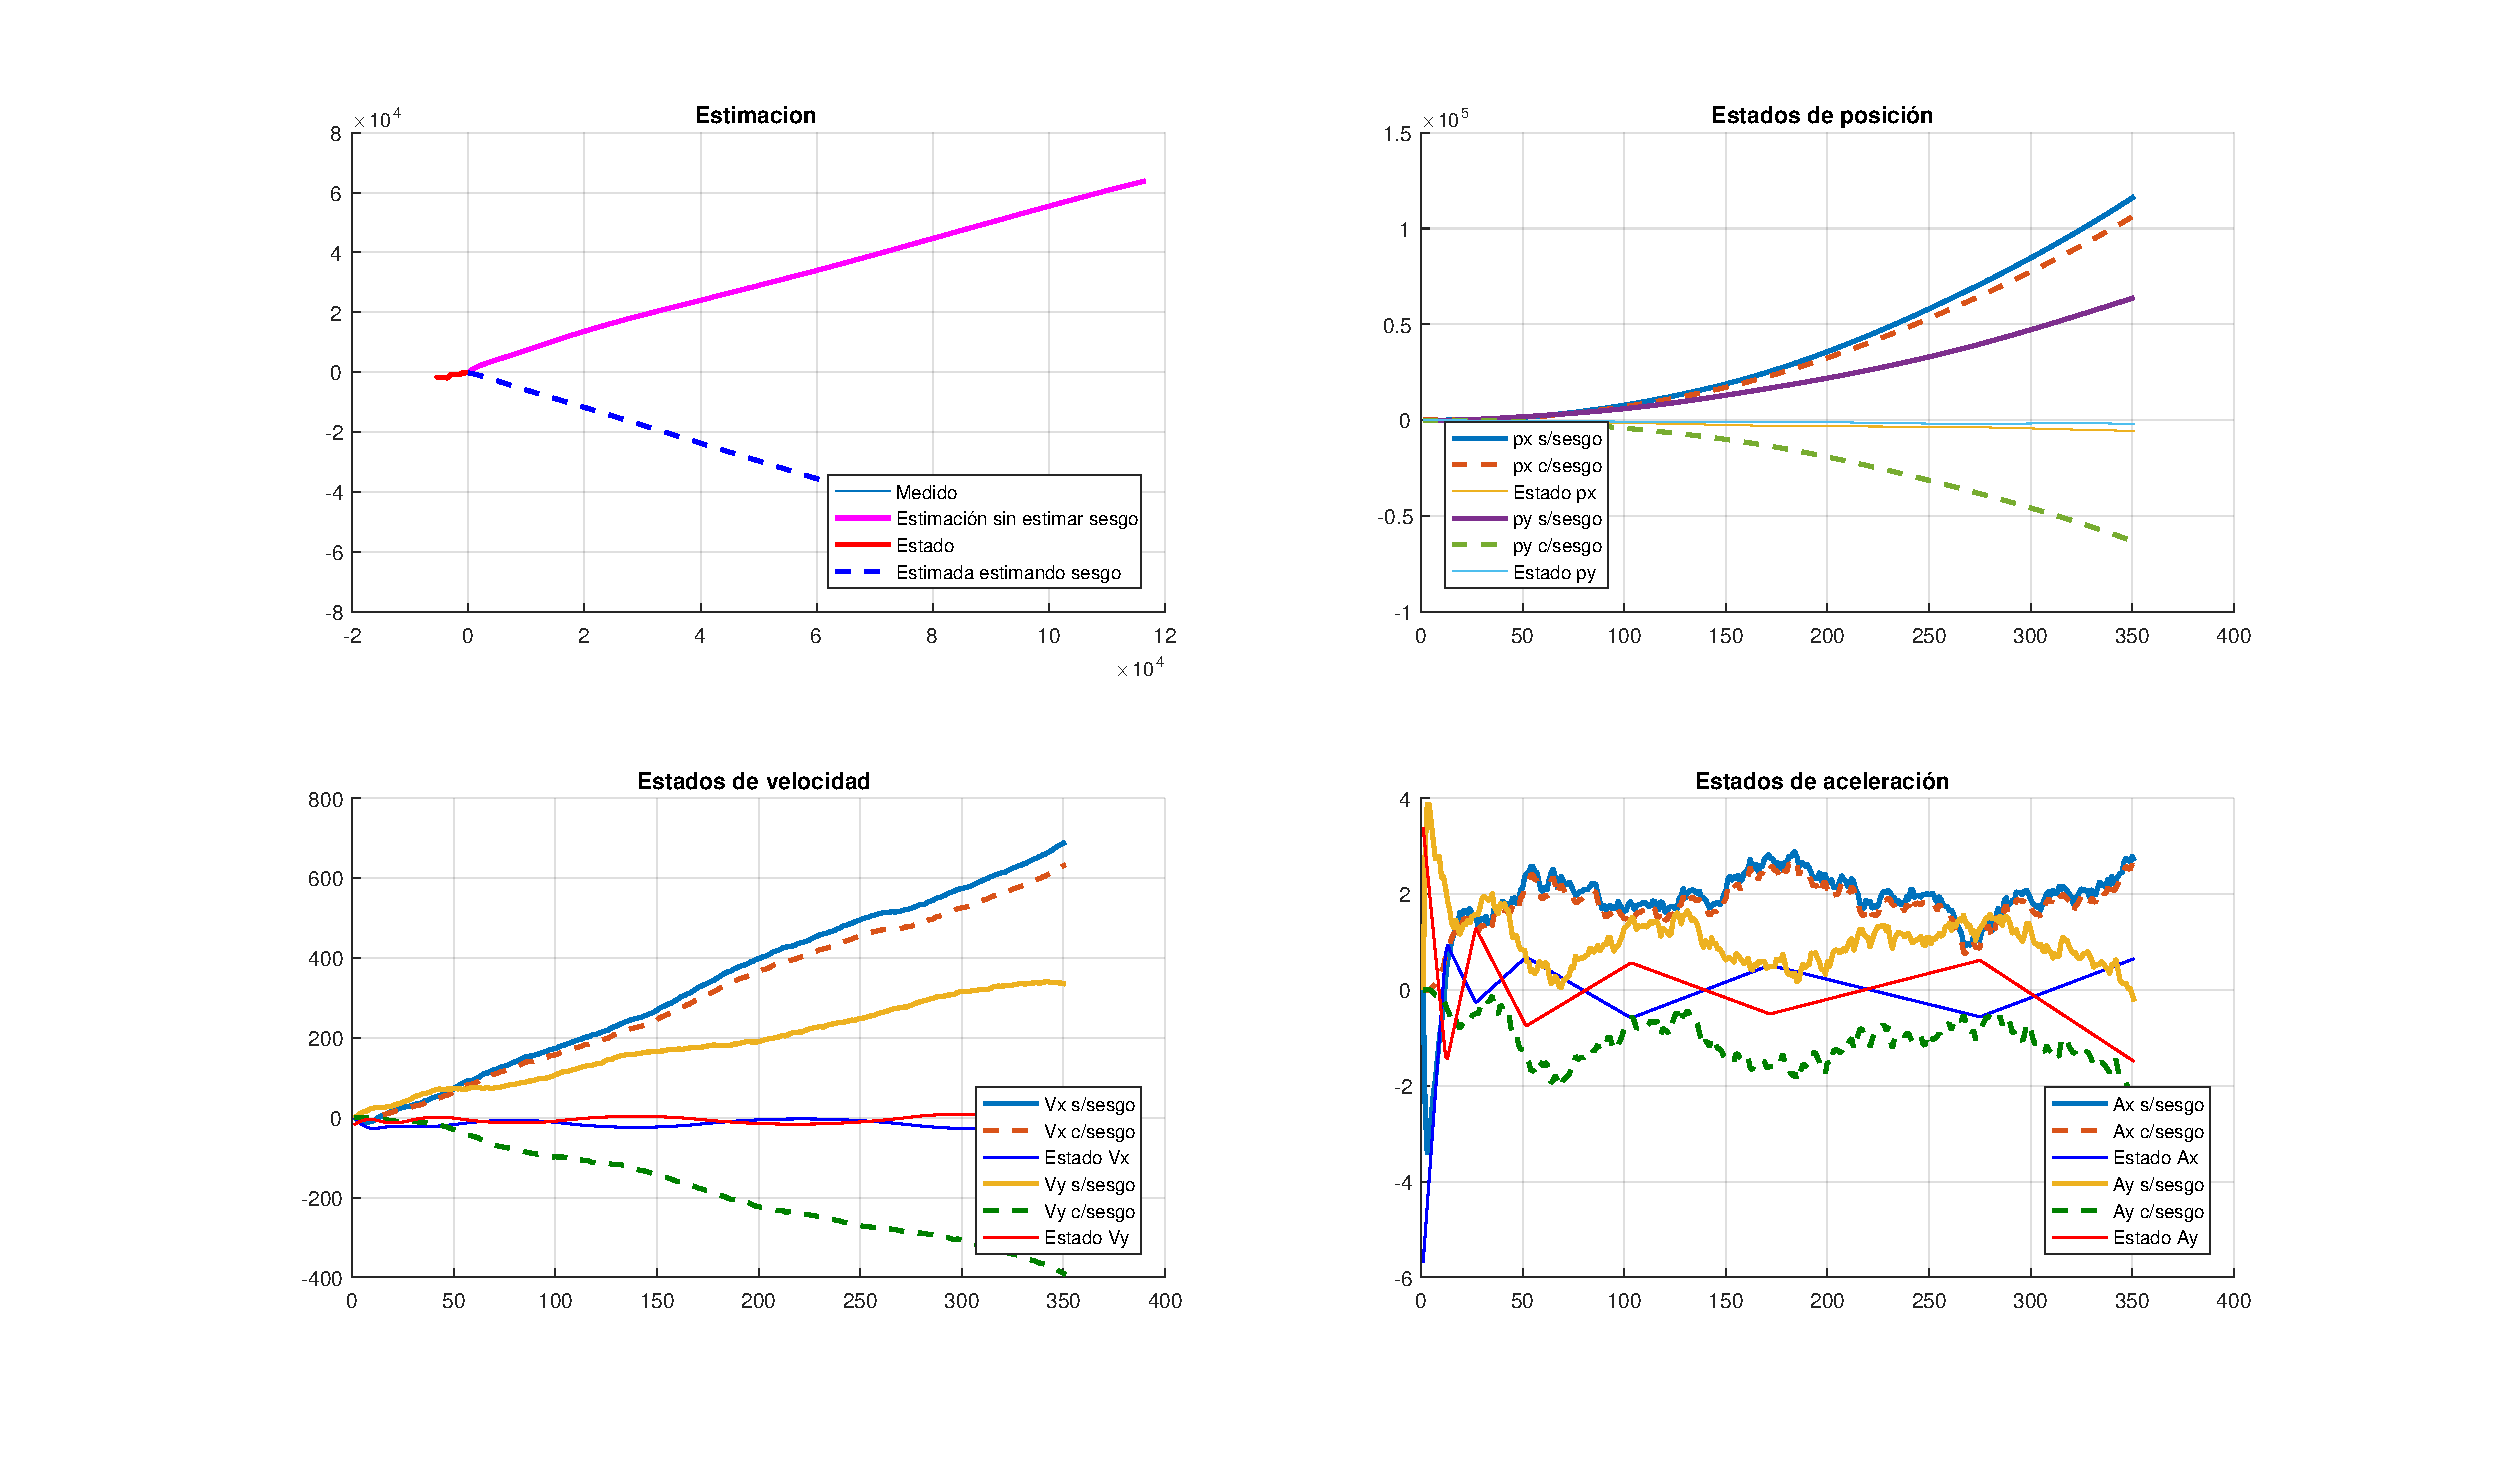
\includegraphics[scale=0.5,trim={6,5cm 0 0 0}]{Figuras/graf_ej4e.pdf}
		\caption{Estimación De Trayectoria}
		\label{fig:ej4e}
	\end{figure}
	
	En la figura \ref{fig:ej4e_bias} podemos observar la convergencia de la estimación. Si bien la misma converge, al no tener observabilidad no lo hace a los valores correctos.
	
	\begin{figure}[H]
		\centering
		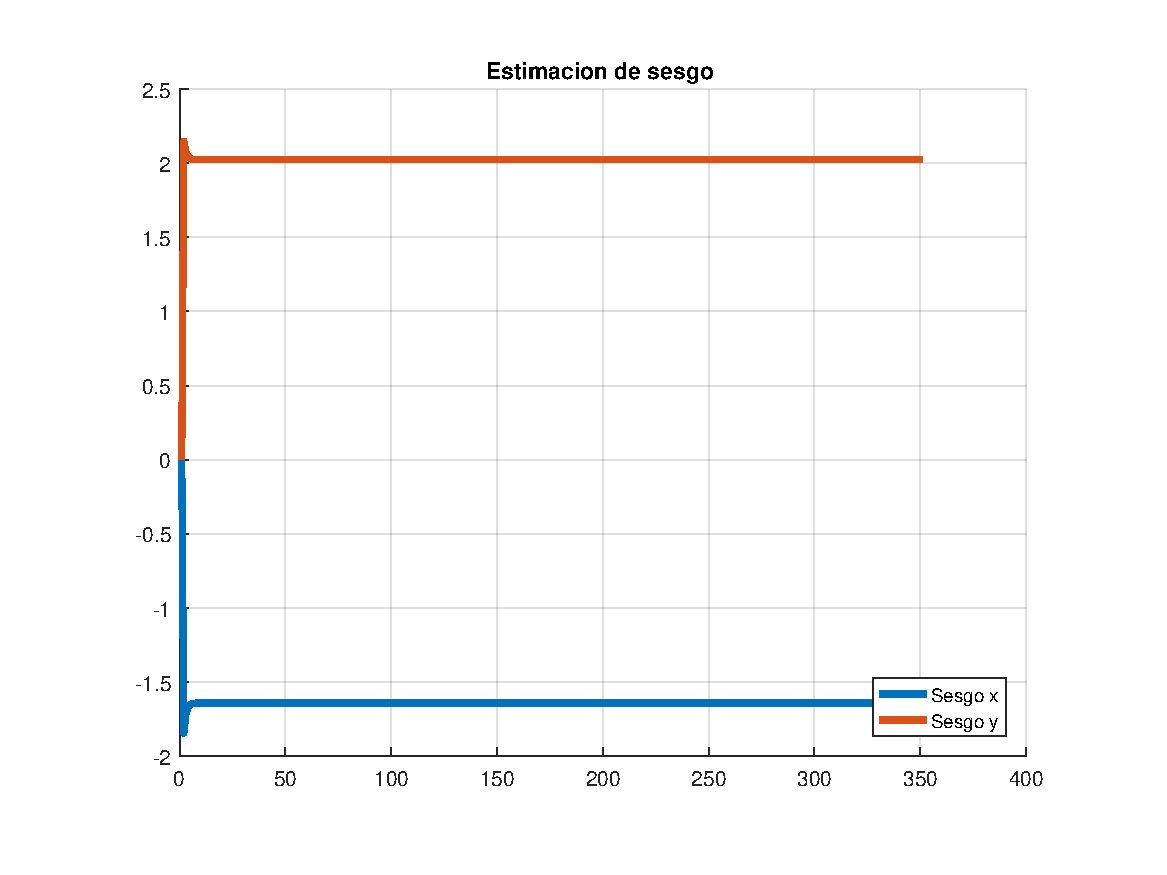
\includegraphics[width=0.7\textwidth,keepaspectratio]{Figuras/bias_ej4e.pdf}
		\caption{Estimación Del Sesgo}
		\label{fig:ej4e_bias}
	\end{figure}
	
	En la figura \ref{fig:ej4e_cov} observamos la autocorrelación de las innovaciones. Puede verse que no se trata de un proceso totalmente blanco.
	
	\begin{figure}[H]
		\centering
		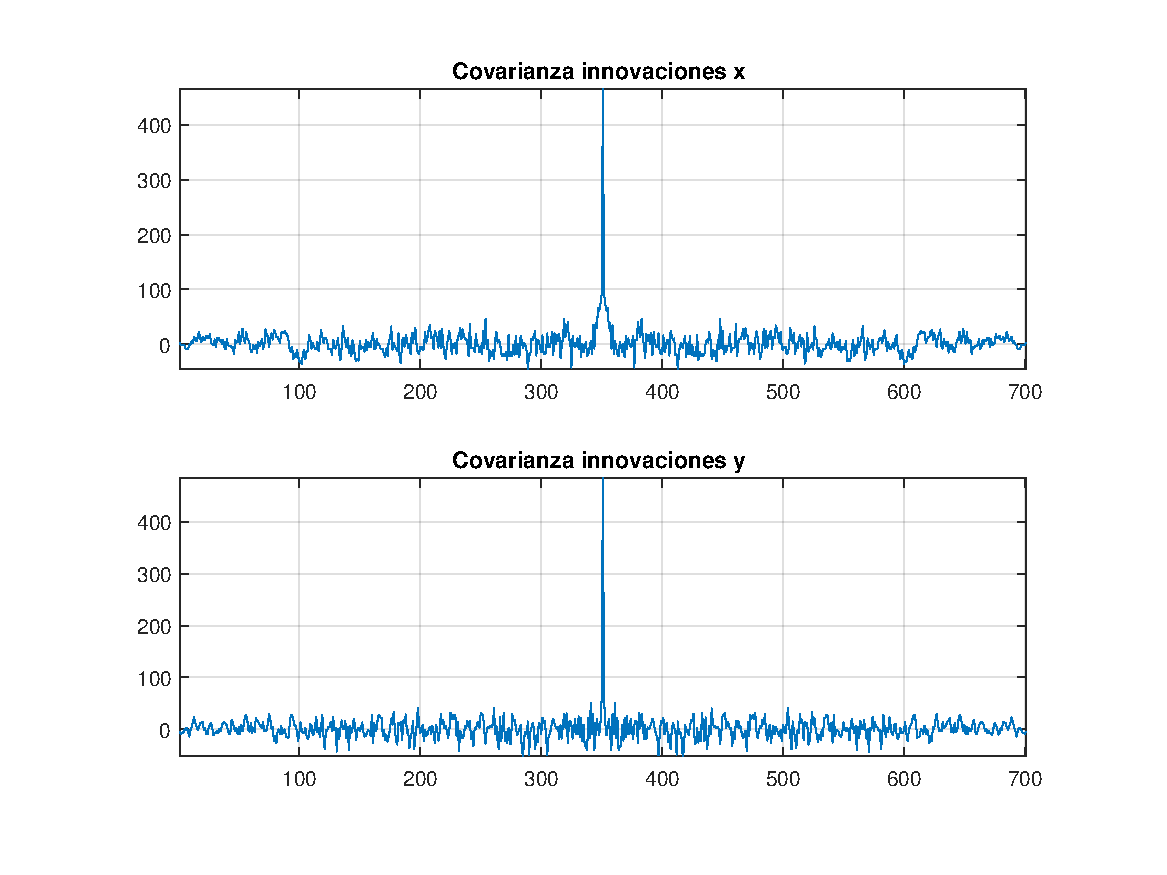
\includegraphics[width=1.0\textwidth,keepaspectratio]{Figuras/covinn_ej4e.pdf}
		\caption{Correlación De Innovaciones}
		\label{fig:ej4e_cov}
	\end{figure}

%--------------------------------------------------------------------------------------------------

\subsection{Medición de PVA - Sesgo en A}

	En la figura \ref{fig:ej3f} se observa el resultado de la estimación. Nuevamente no tenemos problemas de observabilidad, por lo que la estimación sigue la trayectoria y, además, sigue la aceleración de forma correcta.

	\begin{figure}[H]
		\centering
		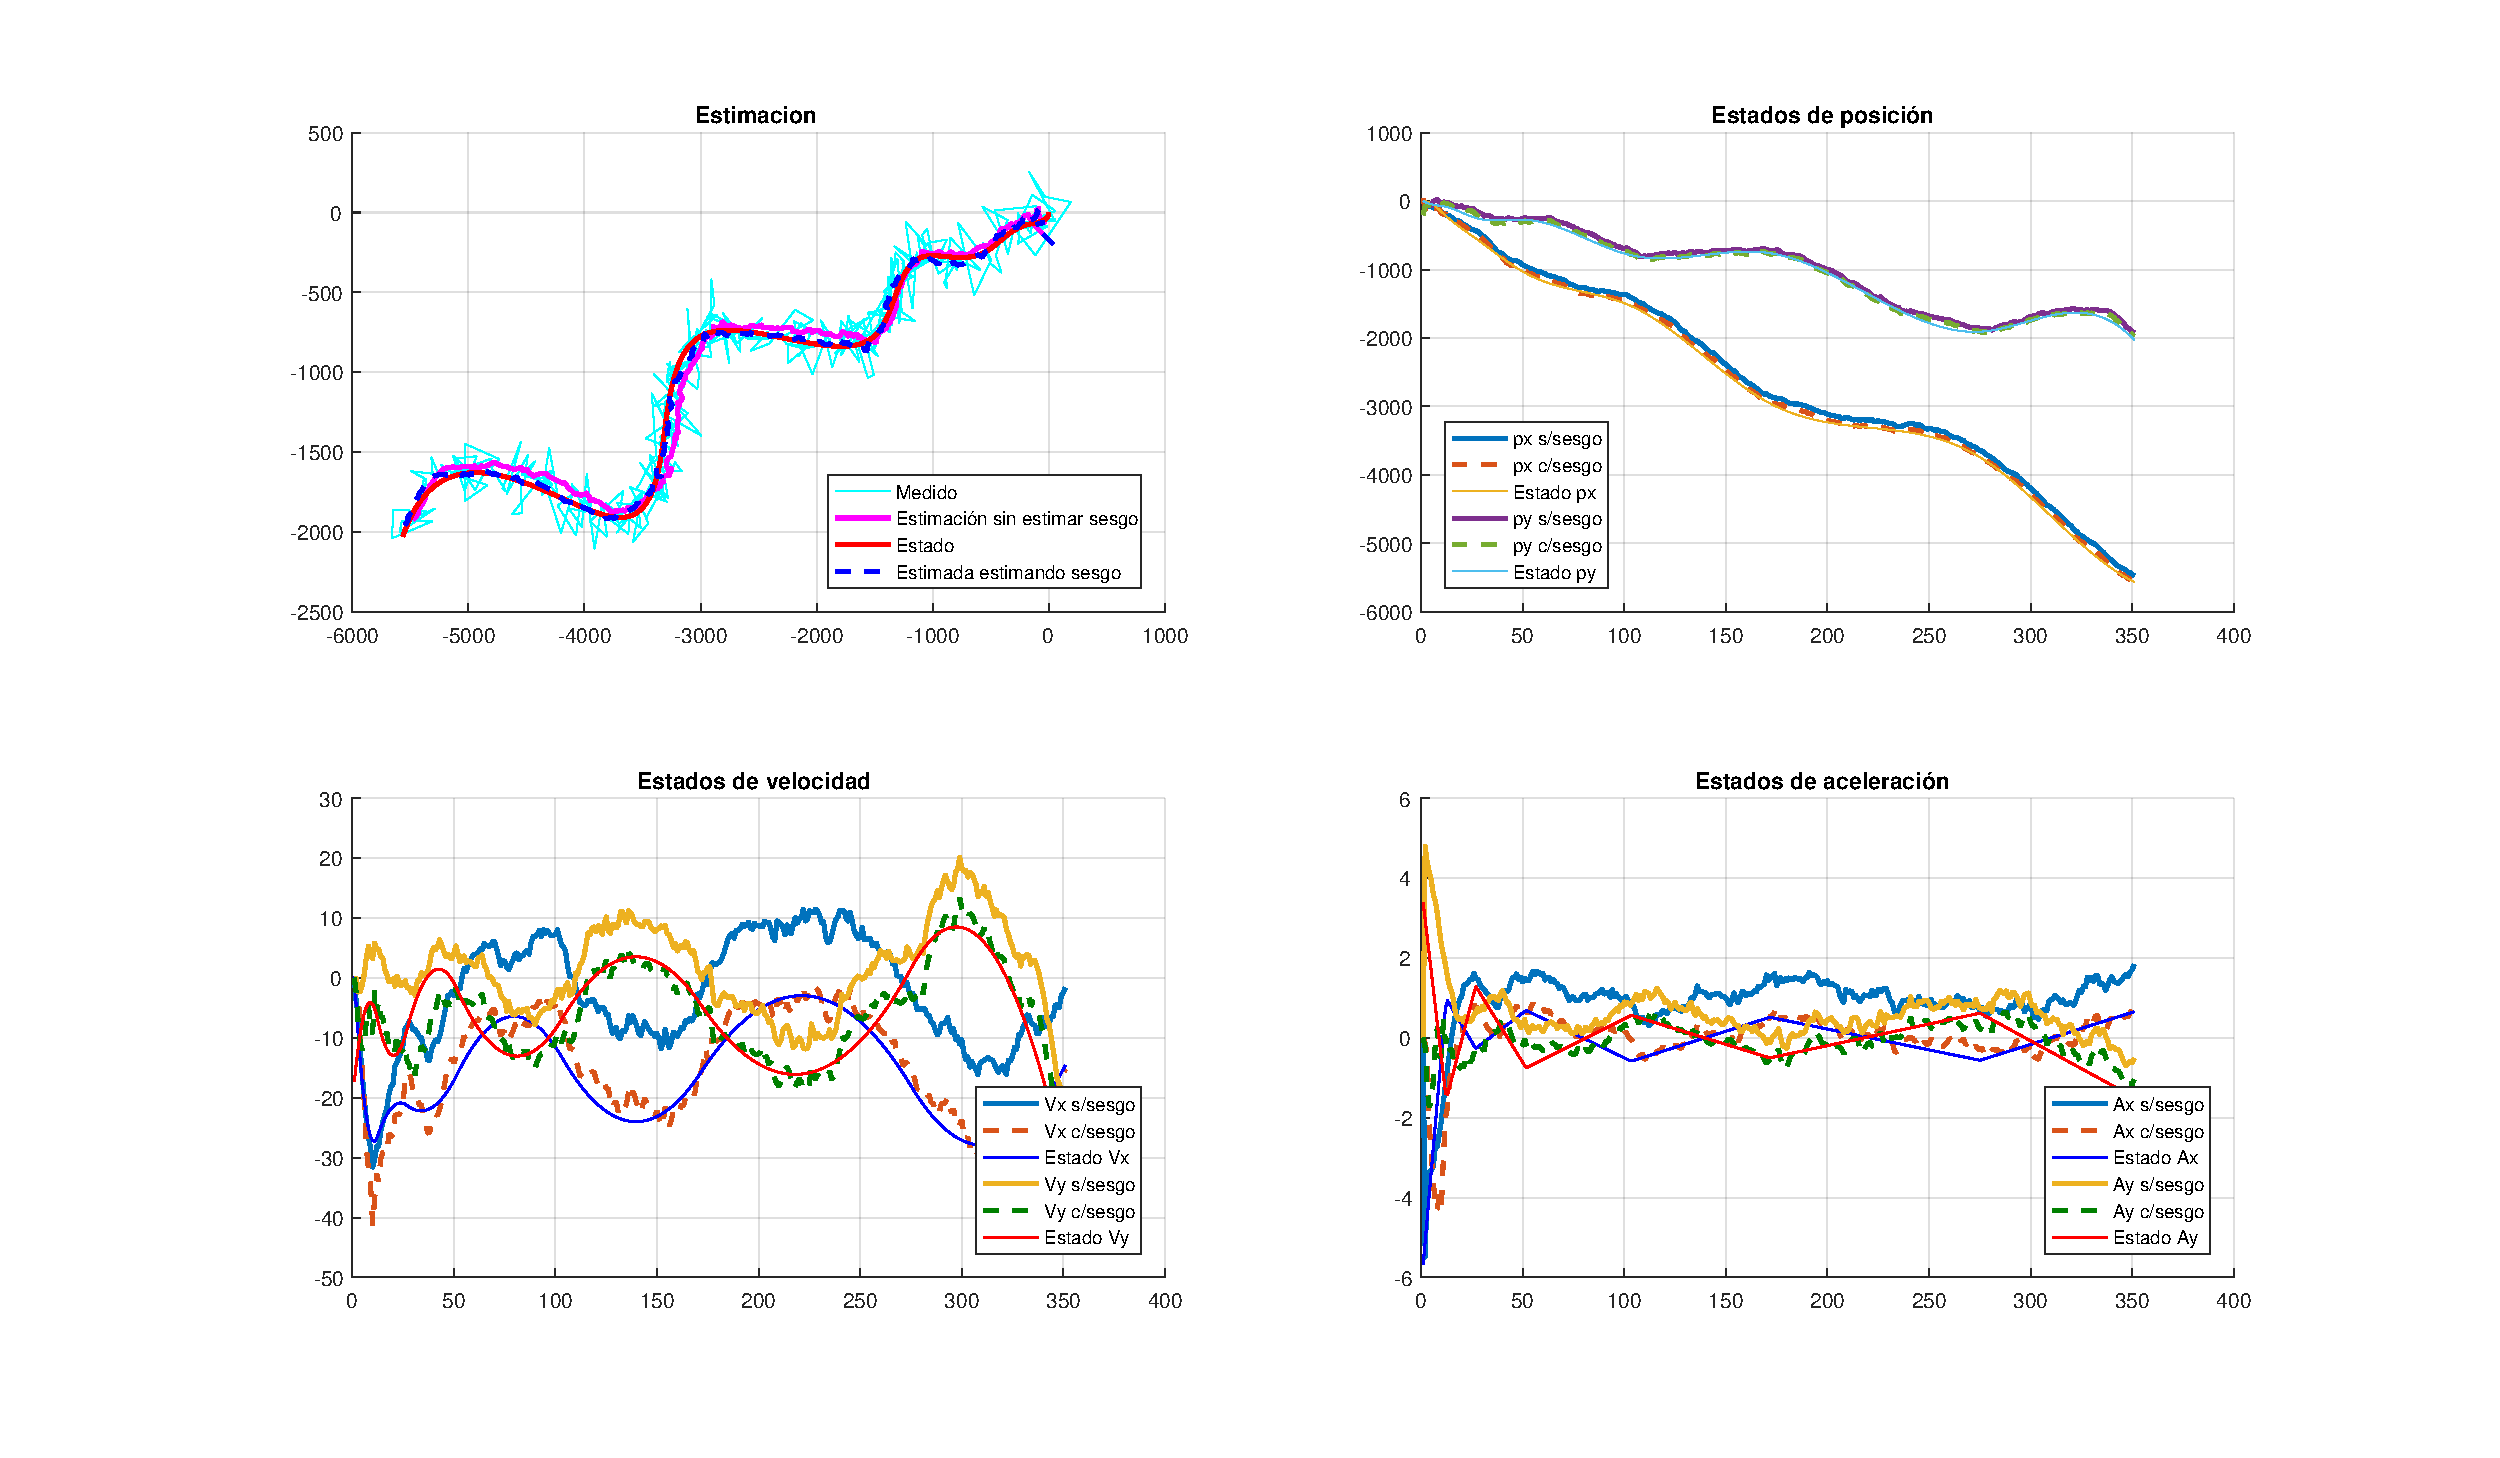
\includegraphics[scale=0.5,trim={6,5cm 0 0 0}]{Figuras/graf_ej4f.pdf}
		\caption{Estimación De Trayectoria}
		\label{fig:ej3f}
	\end{figure}
	
	En la figura \ref{fig:ej3f_bias} se observa la convergencia de la estimación del sesgo. Al tener observabilidad, puede comprobarse que converge a los valores correctos.
	
	\begin{figure}[H]
		\centering
		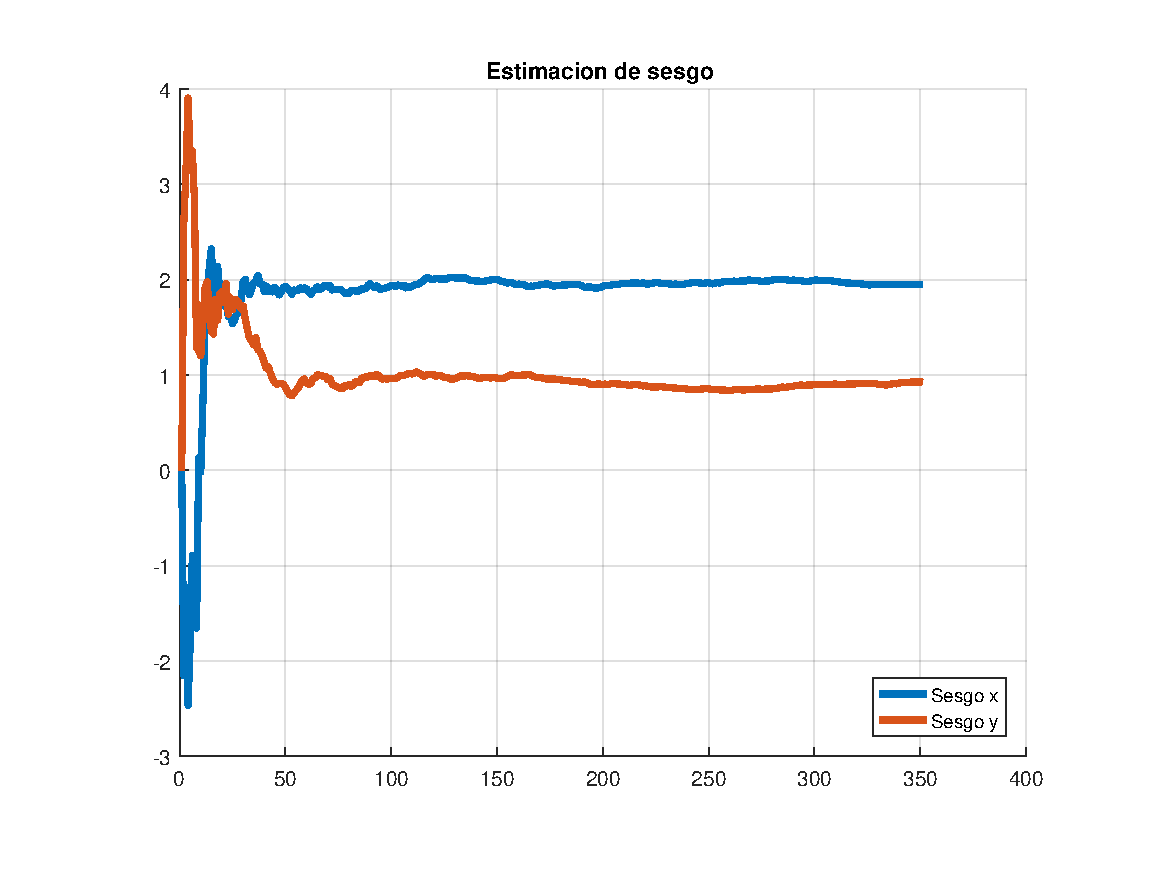
\includegraphics[width=0.7\textwidth,keepaspectratio]{Figuras/bias_ej4f.pdf}
		\caption{Estimación Del Sesgo}
		\label{fig:ej3f_bias}
	\end{figure}
	
	En la figura \ref{fig:ej3f_cov} se observa la autocorrelación de las innovaciones. Puede verse que no se trata de un proceso blanco.

	\begin{figure}[H]
		\centering
		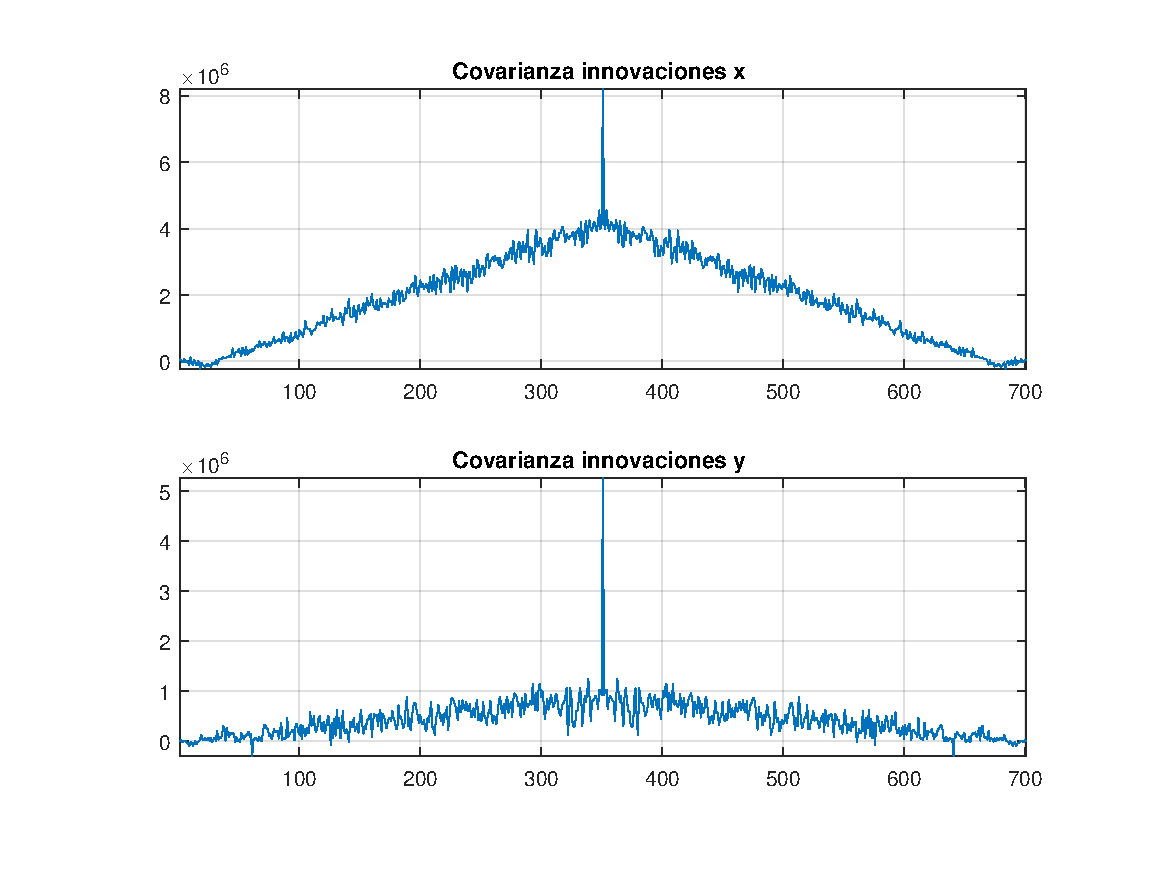
\includegraphics[width=1.0\textwidth,keepaspectratio]{Figuras/covinn_ej4f.pdf}
		\caption{Correlación De Innovaciones}
		\label{fig:ej3f_cov}
	\end{figure}
	
%--------------------------------------------------------------------------------------------------

\subsection{Script}

	A continuación incluimos el script que realiza la estimación. Puede seleccionarse mediante las variables bool\_p, bool\_v, bool\_a, en 1 o en 0, qué se va a medir. Por otro lado puede seleccionarse mediante las variables bool\_pb, bool\_vb, bool\_ab, en 1 o en 0, en qué variables se desea tener sesgo.
	
	%\lstinputlisting[]{../Octave/EJ4a.m}

%--------------------------------------------------------------------------------------------------
